\DeclareUnicodeCharacter{041B}{\CYRL}



\documentclass[11pt]{article}

    
    
    \usepackage[breakable]{tcolorbox}
    \usepackage{parskip} % Stop auto-indenting (to mimic markdown behaviour)
    \usepackage[english,russian]{babel}
    \usepackage{graphicx}
    \usepackage{subcaption}
    

    % Basic figure setup, for now with no caption control since it's done
    % automatically by Pandoc (which extracts ![](path) syntax from Markdown).
    \usepackage{graphicx}
    % Maintain compatibility with old templates. Remove in nbconvert 6.0
    \let\Oldincludegraphics\includegraphics
    % Ensure that by default, figures have no caption (until we provide a
    % proper Figure object with a Caption API and a way to capture that
    % in the conversion process - todo).
    \usepackage{caption}
    \DeclareCaptionFormat{nocaption}{}
    \captionsetup{format=nocaption,aboveskip=0pt,belowskip=0pt}

    \usepackage{float}
    \floatplacement{figure}{H} % forces figures to be placed at the correct location
    \usepackage{xcolor} % Allow colors to be defined
    \usepackage{enumerate} % Needed for markdown enumerations to work
    \usepackage{geometry} % Used to adjust the document margins
    \usepackage{amsmath} % Equations
    \usepackage{amssymb} % Equations
    \usepackage{textcomp} % defines textquotesingle
    % Hack from http://tex.stackexchange.com/a/47451/13684:
    \AtBeginDocument{%
        \def\PYZsq{\textquotesingle}% Upright quotes in Pygmentized code
    }
    \usepackage{upquote} % Upright quotes for verbatim code
    \usepackage{eurosym} % defines \euro

    \usepackage{iftex}
    \ifPDFTeX
        \usepackage[T1]{fontenc}
        \IfFileExists{alphabeta.sty}{
              \usepackage{alphabeta}
          }{
              \usepackage[mathletters]{ucs}
              \usepackage[utf8x]{inputenc}
          }
    \else
        \usepackage{fontspec}
        \usepackage{unicode-math}
    \fi

    \usepackage{fancyvrb} % verbatim replacement that allows latex
    \usepackage{grffile} % extends the file name processing of package graphics
                         % to support a larger range
    \makeatletter % fix for old versions of grffile with XeLaTeX
    \@ifpackagelater{grffile}{2019/11/01}
    {
      % Do nothing on new versions
    }
    {
      \def\Gread@@xetex#1{%
        \IfFileExists{"\Gin@base".bb}%
        {\Gread@eps{\Gin@base.bb}}%
        {\Gread@@xetex@aux#1}%
      }
    }
    \makeatother
    \usepackage[Export]{adjustbox} % Used to constrain images to a maximum size
    \adjustboxset{max size={0.9\linewidth}{0.9\paperheight}}

    % The hyperref package gives us a pdf with properly built
    % internal navigation ('pdf bookmarks' for the table of contents,
    % internal cross-reference links, web links for URLs, etc.)
    \usepackage{hyperref}
    % The default LaTeX title has an obnoxious amount of whitespace. By default,
    % titling removes some of it. It also provides customization options.
    \usepackage{titling}
    \usepackage{longtable} % longtable support required by pandoc >1.10
    \usepackage{booktabs}  % table support for pandoc > 1.12.2
    \usepackage{array}     % table support for pandoc >= 2.11.3
    \usepackage{calc}      % table minipage width calculation for pandoc >= 2.11.1
    \usepackage[inline]{enumitem} % IRkernel/repr support (it uses the enumerate* environment)
    \usepackage[normalem]{ulem} % ulem is needed to support strikethroughs (\sout)
                                % normalem makes italics be italics, not underlines
    \usepackage{mathrsfs}
    

    
    % Colors for the hyperref package
    \definecolor{urlcolor}{rgb}{0,.145,.698}
    \definecolor{linkcolor}{rgb}{.71,0.21,0.01}
    \definecolor{citecolor}{rgb}{.12,.54,.11}

    % ANSI colors
    \definecolor{ansi-black}{HTML}{3E424D}
    \definecolor{ansi-black-intense}{HTML}{282C36}
    \definecolor{ansi-red}{HTML}{E75C58}
    \definecolor{ansi-red-intense}{HTML}{B22B31}
    \definecolor{ansi-green}{HTML}{00A250}
    \definecolor{ansi-green-intense}{HTML}{007427}
    \definecolor{ansi-yellow}{HTML}{DDB62B}
    \definecolor{ansi-yellow-intense}{HTML}{B27D12}
    \definecolor{ansi-blue}{HTML}{208FFB}
    \definecolor{ansi-blue-intense}{HTML}{0065CA}
    \definecolor{ansi-magenta}{HTML}{D160C4}
    \definecolor{ansi-magenta-intense}{HTML}{A03196}
    \definecolor{ansi-cyan}{HTML}{60C6C8}
    \definecolor{ansi-cyan-intense}{HTML}{258F8F}
    \definecolor{ansi-white}{HTML}{C5C1B4}
    \definecolor{ansi-white-intense}{HTML}{A1A6B2}
    \definecolor{ansi-default-inverse-fg}{HTML}{FFFFFF}
    \definecolor{ansi-default-inverse-bg}{HTML}{000000}

    % common color for the border for error outputs.
    \definecolor{outerrorbackground}{HTML}{FFDFDF}

    % commands and environments needed by pandoc snippets
    % extracted from the output of `pandoc -s`
    \providecommand{\tightlist}{%
      \setlength{\itemsep}{0pt}\setlength{\parskip}{0pt}}
    \DefineVerbatimEnvironment{Highlighting}{Verbatim}{commandchars=\\\{\}}
    % Add ',fontsize=\small' for more characters per line
    \newenvironment{Shaded}{}{}
    \newcommand{\KeywordTok}[1]{\textcolor[rgb]{0.00,0.44,0.13}{\textbf{{#1}}}}
    \newcommand{\DataTypeTok}[1]{\textcolor[rgb]{0.56,0.13,0.00}{{#1}}}
    \newcommand{\DecValTok}[1]{\textcolor[rgb]{0.25,0.63,0.44}{{#1}}}
    \newcommand{\BaseNTok}[1]{\textcolor[rgb]{0.25,0.63,0.44}{{#1}}}
    \newcommand{\FloatTok}[1]{\textcolor[rgb]{0.25,0.63,0.44}{{#1}}}
    \newcommand{\CharTok}[1]{\textcolor[rgb]{0.25,0.44,0.63}{{#1}}}
    \newcommand{\StringTok}[1]{\textcolor[rgb]{0.25,0.44,0.63}{{#1}}}
    \newcommand{\CommentTok}[1]{\textcolor[rgb]{0.38,0.63,0.69}{\textit{{#1}}}}
    \newcommand{\OtherTok}[1]{\textcolor[rgb]{0.00,0.44,0.13}{{#1}}}
    \newcommand{\AlertTok}[1]{\textcolor[rgb]{1.00,0.00,0.00}{\textbf{{#1}}}}
    \newcommand{\FunctionTok}[1]{\textcolor[rgb]{0.02,0.16,0.49}{{#1}}}
    \newcommand{\RegionMarkerTok}[1]{{#1}}
    \newcommand{\ErrorTok}[1]{\textcolor[rgb]{1.00,0.00,0.00}{\textbf{{#1}}}}
    \newcommand{\NormalTok}[1]{{#1}}

    % Additional commands for more recent versions of Pandoc
    \newcommand{\ConstantTok}[1]{\textcolor[rgb]{0.53,0.00,0.00}{{#1}}}
    \newcommand{\SpecialCharTok}[1]{\textcolor[rgb]{0.25,0.44,0.63}{{#1}}}
    \newcommand{\VerbatimStringTok}[1]{\textcolor[rgb]{0.25,0.44,0.63}{{#1}}}
    \newcommand{\SpecialStringTok}[1]{\textcolor[rgb]{0.73,0.40,0.53}{{#1}}}
    \newcommand{\ImportTok}[1]{{#1}}
    \newcommand{\DocumentationTok}[1]{\textcolor[rgb]{0.73,0.13,0.13}{\textit{{#1}}}}
    \newcommand{\AnnotationTok}[1]{\textcolor[rgb]{0.38,0.63,0.69}{\textbf{\textit{{#1}}}}}
    \newcommand{\CommentVarTok}[1]{\textcolor[rgb]{0.38,0.63,0.69}{\textbf{\textit{{#1}}}}}
    \newcommand{\VariableTok}[1]{\textcolor[rgb]{0.10,0.09,0.49}{{#1}}}
    \newcommand{\ControlFlowTok}[1]{\textcolor[rgb]{0.00,0.44,0.13}{\textbf{{#1}}}}
    \newcommand{\OperatorTok}[1]{\textcolor[rgb]{0.40,0.40,0.40}{{#1}}}
    \newcommand{\BuiltInTok}[1]{{#1}}
    \newcommand{\ExtensionTok}[1]{{#1}}
    \newcommand{\PreprocessorTok}[1]{\textcolor[rgb]{0.74,0.48,0.00}{{#1}}}
    \newcommand{\AttributeTok}[1]{\textcolor[rgb]{0.49,0.56,0.16}{{#1}}}
    \newcommand{\InformationTok}[1]{\textcolor[rgb]{0.38,0.63,0.69}{\textbf{\textit{{#1}}}}}
    \newcommand{\WarningTok}[1]{\textcolor[rgb]{0.38,0.63,0.69}{\textbf{\textit{{#1}}}}}


    % Define a nice break command that doesn't care if a line doesn't already
    % exist.
    \def\br{\hspace*{\fill} \\* }
    % Math Jax compatibility definitions
    \def\gt{>}
    \def\lt{<}
    \let\Oldtex\TeX
    \let\Oldlatex\LaTeX
    \renewcommand{\TeX}{\textrm{\Oldtex}}
    \renewcommand{\LaTeX}{\textrm{\Oldlatex}}
    % Document parameters
    % Document title
    \title{CHM\_Lab1}
    
    
    
    
    
% Pygments definitions
\makeatletter
\def\PY@reset{\let\PY@it=\relax \let\PY@bf=\relax%
    \let\PY@ul=\relax \let\PY@tc=\relax%
    \let\PY@bc=\relax \let\PY@ff=\relax}
\def\PY@tok#1{\csname PY@tok@#1\endcsname}
\def\PY@toks#1+{\ifx\relax#1\empty\else%
    \PY@tok{#1}\expandafter\PY@toks\fi}
\def\PY@do#1{\PY@bc{\PY@tc{\PY@ul{%
    \PY@it{\PY@bf{\PY@ff{#1}}}}}}}
\def\PY#1#2{\PY@reset\PY@toks#1+\relax+\PY@do{#2}}

\@namedef{PY@tok@w}{\def\PY@tc##1{\textcolor[rgb]{0.73,0.73,0.73}{##1}}}
\@namedef{PY@tok@c}{\let\PY@it=\textit\def\PY@tc##1{\textcolor[rgb]{0.24,0.48,0.48}{##1}}}
\@namedef{PY@tok@cp}{\def\PY@tc##1{\textcolor[rgb]{0.61,0.40,0.00}{##1}}}
\@namedef{PY@tok@k}{\let\PY@bf=\textbf\def\PY@tc##1{\textcolor[rgb]{0.00,0.50,0.00}{##1}}}
\@namedef{PY@tok@kp}{\def\PY@tc##1{\textcolor[rgb]{0.00,0.50,0.00}{##1}}}
\@namedef{PY@tok@kt}{\def\PY@tc##1{\textcolor[rgb]{0.69,0.00,0.25}{##1}}}
\@namedef{PY@tok@o}{\def\PY@tc##1{\textcolor[rgb]{0.40,0.40,0.40}{##1}}}
\@namedef{PY@tok@ow}{\let\PY@bf=\textbf\def\PY@tc##1{\textcolor[rgb]{0.67,0.13,1.00}{##1}}}
\@namedef{PY@tok@nb}{\def\PY@tc##1{\textcolor[rgb]{0.00,0.50,0.00}{##1}}}
\@namedef{PY@tok@nf}{\def\PY@tc##1{\textcolor[rgb]{0.00,0.00,1.00}{##1}}}
\@namedef{PY@tok@nc}{\let\PY@bf=\textbf\def\PY@tc##1{\textcolor[rgb]{0.00,0.00,1.00}{##1}}}
\@namedef{PY@tok@nn}{\let\PY@bf=\textbf\def\PY@tc##1{\textcolor[rgb]{0.00,0.00,1.00}{##1}}}
\@namedef{PY@tok@ne}{\let\PY@bf=\textbf\def\PY@tc##1{\textcolor[rgb]{0.80,0.25,0.22}{##1}}}
\@namedef{PY@tok@nv}{\def\PY@tc##1{\textcolor[rgb]{0.10,0.09,0.49}{##1}}}
\@namedef{PY@tok@no}{\def\PY@tc##1{\textcolor[rgb]{0.53,0.00,0.00}{##1}}}
\@namedef{PY@tok@nl}{\def\PY@tc##1{\textcolor[rgb]{0.46,0.46,0.00}{##1}}}
\@namedef{PY@tok@ni}{\let\PY@bf=\textbf\def\PY@tc##1{\textcolor[rgb]{0.44,0.44,0.44}{##1}}}
\@namedef{PY@tok@na}{\def\PY@tc##1{\textcolor[rgb]{0.41,0.47,0.13}{##1}}}
\@namedef{PY@tok@nt}{\let\PY@bf=\textbf\def\PY@tc##1{\textcolor[rgb]{0.00,0.50,0.00}{##1}}}
\@namedef{PY@tok@nd}{\def\PY@tc##1{\textcolor[rgb]{0.67,0.13,1.00}{##1}}}
\@namedef{PY@tok@s}{\def\PY@tc##1{\textcolor[rgb]{0.73,0.13,0.13}{##1}}}
\@namedef{PY@tok@sd}{\let\PY@it=\textit\def\PY@tc##1{\textcolor[rgb]{0.73,0.13,0.13}{##1}}}
\@namedef{PY@tok@si}{\let\PY@bf=\textbf\def\PY@tc##1{\textcolor[rgb]{0.64,0.35,0.47}{##1}}}
\@namedef{PY@tok@se}{\let\PY@bf=\textbf\def\PY@tc##1{\textcolor[rgb]{0.67,0.36,0.12}{##1}}}
\@namedef{PY@tok@sr}{\def\PY@tc##1{\textcolor[rgb]{0.64,0.35,0.47}{##1}}}
\@namedef{PY@tok@ss}{\def\PY@tc##1{\textcolor[rgb]{0.10,0.09,0.49}{##1}}}
\@namedef{PY@tok@sx}{\def\PY@tc##1{\textcolor[rgb]{0.00,0.50,0.00}{##1}}}
\@namedef{PY@tok@m}{\def\PY@tc##1{\textcolor[rgb]{0.40,0.40,0.40}{##1}}}
\@namedef{PY@tok@gh}{\let\PY@bf=\textbf\def\PY@tc##1{\textcolor[rgb]{0.00,0.00,0.50}{##1}}}
\@namedef{PY@tok@gu}{\let\PY@bf=\textbf\def\PY@tc##1{\textcolor[rgb]{0.50,0.00,0.50}{##1}}}
\@namedef{PY@tok@gd}{\def\PY@tc##1{\textcolor[rgb]{0.63,0.00,0.00}{##1}}}
\@namedef{PY@tok@gi}{\def\PY@tc##1{\textcolor[rgb]{0.00,0.52,0.00}{##1}}}
\@namedef{PY@tok@gr}{\def\PY@tc##1{\textcolor[rgb]{0.89,0.00,0.00}{##1}}}
\@namedef{PY@tok@ge}{\let\PY@it=\textit}
\@namedef{PY@tok@gs}{\let\PY@bf=\textbf}
\@namedef{PY@tok@gp}{\let\PY@bf=\textbf\def\PY@tc##1{\textcolor[rgb]{0.00,0.00,0.50}{##1}}}
\@namedef{PY@tok@go}{\def\PY@tc##1{\textcolor[rgb]{0.44,0.44,0.44}{##1}}}
\@namedef{PY@tok@gt}{\def\PY@tc##1{\textcolor[rgb]{0.00,0.27,0.87}{##1}}}
\@namedef{PY@tok@err}{\def\PY@bc##1{{\setlength{\fboxsep}{\string -\fboxrule}\fcolorbox[rgb]{1.00,0.00,0.00}{1,1,1}{\strut ##1}}}}
\@namedef{PY@tok@kc}{\let\PY@bf=\textbf\def\PY@tc##1{\textcolor[rgb]{0.00,0.50,0.00}{##1}}}
\@namedef{PY@tok@kd}{\let\PY@bf=\textbf\def\PY@tc##1{\textcolor[rgb]{0.00,0.50,0.00}{##1}}}
\@namedef{PY@tok@kn}{\let\PY@bf=\textbf\def\PY@tc##1{\textcolor[rgb]{0.00,0.50,0.00}{##1}}}
\@namedef{PY@tok@kr}{\let\PY@bf=\textbf\def\PY@tc##1{\textcolor[rgb]{0.00,0.50,0.00}{##1}}}
\@namedef{PY@tok@bp}{\def\PY@tc##1{\textcolor[rgb]{0.00,0.50,0.00}{##1}}}
\@namedef{PY@tok@fm}{\def\PY@tc##1{\textcolor[rgb]{0.00,0.00,1.00}{##1}}}
\@namedef{PY@tok@vc}{\def\PY@tc##1{\textcolor[rgb]{0.10,0.09,0.49}{##1}}}
\@namedef{PY@tok@vg}{\def\PY@tc##1{\textcolor[rgb]{0.10,0.09,0.49}{##1}}}
\@namedef{PY@tok@vi}{\def\PY@tc##1{\textcolor[rgb]{0.10,0.09,0.49}{##1}}}
\@namedef{PY@tok@vm}{\def\PY@tc##1{\textcolor[rgb]{0.10,0.09,0.49}{##1}}}
\@namedef{PY@tok@sa}{\def\PY@tc##1{\textcolor[rgb]{0.73,0.13,0.13}{##1}}}
\@namedef{PY@tok@sb}{\def\PY@tc##1{\textcolor[rgb]{0.73,0.13,0.13}{##1}}}
\@namedef{PY@tok@sc}{\def\PY@tc##1{\textcolor[rgb]{0.73,0.13,0.13}{##1}}}
\@namedef{PY@tok@dl}{\def\PY@tc##1{\textcolor[rgb]{0.73,0.13,0.13}{##1}}}
\@namedef{PY@tok@s2}{\def\PY@tc##1{\textcolor[rgb]{0.73,0.13,0.13}{##1}}}
\@namedef{PY@tok@sh}{\def\PY@tc##1{\textcolor[rgb]{0.73,0.13,0.13}{##1}}}
\@namedef{PY@tok@s1}{\def\PY@tc##1{\textcolor[rgb]{0.73,0.13,0.13}{##1}}}
\@namedef{PY@tok@mb}{\def\PY@tc##1{\textcolor[rgb]{0.40,0.40,0.40}{##1}}}
\@namedef{PY@tok@mf}{\def\PY@tc##1{\textcolor[rgb]{0.40,0.40,0.40}{##1}}}
\@namedef{PY@tok@mh}{\def\PY@tc##1{\textcolor[rgb]{0.40,0.40,0.40}{##1}}}
\@namedef{PY@tok@mi}{\def\PY@tc##1{\textcolor[rgb]{0.40,0.40,0.40}{##1}}}
\@namedef{PY@tok@il}{\def\PY@tc##1{\textcolor[rgb]{0.40,0.40,0.40}{##1}}}
\@namedef{PY@tok@mo}{\def\PY@tc##1{\textcolor[rgb]{0.40,0.40,0.40}{##1}}}
\@namedef{PY@tok@ch}{\let\PY@it=\textit\def\PY@tc##1{\textcolor[rgb]{0.24,0.48,0.48}{##1}}}
\@namedef{PY@tok@cm}{\let\PY@it=\textit\def\PY@tc##1{\textcolor[rgb]{0.24,0.48,0.48}{##1}}}
\@namedef{PY@tok@cpf}{\let\PY@it=\textit\def\PY@tc##1{\textcolor[rgb]{0.24,0.48,0.48}{##1}}}
\@namedef{PY@tok@c1}{\let\PY@it=\textit\def\PY@tc##1{\textcolor[rgb]{0.24,0.48,0.48}{##1}}}
\@namedef{PY@tok@cs}{\let\PY@it=\textit\def\PY@tc##1{\textcolor[rgb]{0.24,0.48,0.48}{##1}}}

\def\PYZbs{\char`\\}
\def\PYZus{\char`\_}
\def\PYZob{\char`\{}
\def\PYZcb{\char`\}}
\def\PYZca{\char`\^}
\def\PYZam{\char`\&}
\def\PYZlt{\char`\<}
\def\PYZgt{\char`\>}
\def\PYZsh{\char`\#}
\def\PYZpc{\char`\%}
\def\PYZdl{\char`\$}
\def\PYZhy{\char`\-}
\def\PYZsq{\char`\'}
\def\PYZdq{\char`\"}
\def\PYZti{\char`\~}
% for compatibility with earlier versions
\def\PYZat{@}
\def\PYZlb{[}
\def\PYZrb{]}
\makeatother


    % For linebreaks inside Verbatim environment from package fancyvrb.
    \makeatletter
        \newbox\Wrappedcontinuationbox
        \newbox\Wrappedvisiblespacebox
        \newcommand*\Wrappedvisiblespace {\textcolor{red}{\textvisiblespace}}
        \newcommand*\Wrappedcontinuationsymbol {\textcolor{red}{\llap{\tiny$\m@th\hookrightarrow$}}}
        \newcommand*\Wrappedcontinuationindent {3ex }
        \newcommand*\Wrappedafterbreak {\kern\Wrappedcontinuationindent\copy\Wrappedcontinuationbox}
        % Take advantage of the already applied Pygments mark-up to insert
        % potential linebreaks for TeX processing.
        %        {, <, #, %, $, ' and ": go to next line.
        %        _, }, ^, &, >, - and ~: stay at end of broken line.
        % Use of \textquotesingle for straight quote.
        \newcommand*\Wrappedbreaksatspecials {%
            \def\PYGZus{\discretionary{\char`\_}{\Wrappedafterbreak}{\char`\_}}%
            \def\PYGZob{\discretionary{}{\Wrappedafterbreak\char`\{}{\char`\{}}%
            \def\PYGZcb{\discretionary{\char`\}}{\Wrappedafterbreak}{\char`\}}}%
            \def\PYGZca{\discretionary{\char`\^}{\Wrappedafterbreak}{\char`\^}}%
            \def\PYGZam{\discretionary{\char`\&}{\Wrappedafterbreak}{\char`\&}}%
            \def\PYGZlt{\discretionary{}{\Wrappedafterbreak\char`\<}{\char`\<}}%
            \def\PYGZgt{\discretionary{\char`\>}{\Wrappedafterbreak}{\char`\>}}%
            \def\PYGZsh{\discretionary{}{\Wrappedafterbreak\char`\#}{\char`\#}}%
            \def\PYGZpc{\discretionary{}{\Wrappedafterbreak\char`\%}{\char`\%}}%
            \def\PYGZdl{\discretionary{}{\Wrappedafterbreak\char`\$}{\char`\$}}%
            \def\PYGZhy{\discretionary{\char`\-}{\Wrappedafterbreak}{\char`\-}}%
            \def\PYGZsq{\discretionary{}{\Wrappedafterbreak\textquotesingle}{\textquotesingle}}%
            \def\PYGZdq{\discretionary{}{\Wrappedafterbreak\char`\"}{\char`\"}}%
            \def\PYGZti{\discretionary{\char`\~}{\Wrappedafterbreak}{\char`\~}}%
        }
        % Some characters . , ; ? ! / are not pygmentized.
        % This macro makes them "active" and they will insert potential linebreaks
        \newcommand*\Wrappedbreaksatpunct {%
            \lccode`\~`\.\lowercase{\def~}{\discretionary{\hbox{\char`\.}}{\Wrappedafterbreak}{\hbox{\char`\.}}}%
            \lccode`\~`\,\lowercase{\def~}{\discretionary{\hbox{\char`\,}}{\Wrappedafterbreak}{\hbox{\char`\,}}}%
            \lccode`\~`\;\lowercase{\def~}{\discretionary{\hbox{\char`\;}}{\Wrappedafterbreak}{\hbox{\char`\;}}}%
            \lccode`\~`\:\lowercase{\def~}{\discretionary{\hbox{\char`\:}}{\Wrappedafterbreak}{\hbox{\char`\:}}}%
            \lccode`\~`\?\lowercase{\def~}{\discretionary{\hbox{\char`\?}}{\Wrappedafterbreak}{\hbox{\char`\?}}}%
            \lccode`\~`\!\lowercase{\def~}{\discretionary{\hbox{\char`\!}}{\Wrappedafterbreak}{\hbox{\char`\!}}}%
            \lccode`\~`\/\lowercase{\def~}{\discretionary{\hbox{\char`\/}}{\Wrappedafterbreak}{\hbox{\char`\/}}}%
            \catcode`\.\active
            \catcode`\,\active
            \catcode`\;\active
            \catcode`\:\active
            \catcode`\?\active
            \catcode`\!\active
            \catcode`\/\active
            \lccode`\~`\~
        }
    \makeatother

    \let\OriginalVerbatim=\Verbatim
    \makeatletter
    \renewcommand{\Verbatim}[1][1]{%
        %\parskip\z@skip
        \sbox\Wrappedcontinuationbox {\Wrappedcontinuationsymbol}%
        \sbox\Wrappedvisiblespacebox {\FV@SetupFont\Wrappedvisiblespace}%
        \def\FancyVerbFormatLine ##1{\hsize\linewidth
            \vtop{\raggedright\hyphenpenalty\z@\exhyphenpenalty\z@
                \doublehyphendemerits\z@\finalhyphendemerits\z@
                \strut ##1\strut}%
        }%
        % If the linebreak is at a space, the latter will be displayed as visible
        % space at end of first line, and a continuation symbol starts next line.
        % Stretch/shrink are however usually zero for typewriter font.
        \def\FV@Space {%
            \nobreak\hskip\z@ plus\fontdimen3\font minus\fontdimen4\font
            \discretionary{\copy\Wrappedvisiblespacebox}{\Wrappedafterbreak}
            {\kern\fontdimen2\font}%
        }%

        % Allow breaks at special characters using \PYG... macros.
        \Wrappedbreaksatspecials
        % Breaks at punctuation characters . , ; ? ! and / need catcode=\active
        \OriginalVerbatim[#1,codes*=\Wrappedbreaksatpunct]%
    }
    \makeatother

    % Exact colors from NB
    \definecolor{incolor}{HTML}{303F9F}
    \definecolor{outcolor}{HTML}{D84315}
    \definecolor{cellborder}{HTML}{CFCFCF}
    \definecolor{cellbackground}{HTML}{F7F7F7}

    % prompt
    \makeatletter
    \newcommand{\boxspacing}{\kern\kvtcb@left@rule\kern\kvtcb@boxsep}
    \makeatother
    \newcommand{\prompt}[4]{
        {\ttfamily\llap{{\color{#2}[#3]:\hspace{3pt}#4}}\vspace{-\baselineskip}}
    }
    

    
    % Prevent overflowing lines due to hard-to-break entities
    \sloppy
    % Setup hyperref package
    \hypersetup{
      breaklinks=true,  % so long urls are correctly broken across lines
      colorlinks=true,
      urlcolor=urlcolor,
      linkcolor=linkcolor,
      citecolor=citecolor,
      }
    % Slightly bigger margins than the latex defaults
    
    \geometry{verbose,tmargin=1in,bmargin=1in,lmargin=1in,rmargin=1in}
    
\newtheorem{theorem}{Теорема}

\begin{document}
    
    \begin{titlepage}
    \newpage
    
    \begin{center}
    МИНИСТЕРСТВО ОБРАЗОВАНИЯ РЕСПУБЛИКИ БЕЛАРУСЬ БЕЛОРУССКИЙ ГОСУДАРСТВЕННЫЙ УНИВЕРСИТЕТ \\
    Факультет прикладной математики и инворматики \\ Кафедра вычислительной математики
 
    \end{center}
    
    \vspace{8em}
    
    \vspace{2em}
    
    \begin{center}
    \textsc{\textbf{Отчет по лабораторной работе 3 \\ "Интерполирование функций" \linebreak Вариант 5}}
    \end{center}
    
    \vspace{6em}
    
    \begin{flushright}
        Выполнил:\\
        Карпович Артём Дмитриевич\\
        студент 3 курса 7 группы
    \end{flushright}
    
    \begin{flushright}
        Преподаватель:\\
        Репников Василий Иванович
    \end{flushright}
    
    \vspace{\fill}
    
    \vspace{\fill}
    
    \begin{center}
    Минск, 2024
    \end{center}
    
    \end{titlepage}
    
    \subsection*{Задача 1}

На отрезке \([a, b]=[0, 2]\) задана таблица значений функции \(f(x)\) с
шагом \(h = \frac{1}{10}\). Погрешность каждого заданного значения не
превышает \(e = 10^{-4}\). Используя интерполирования Ньютона для начала
и конца таблицы, с помощью многочленов минимальной степени построить
таблицу значений функции \[f(x)=x\ln{(x+2)}\] с шагом
\(0.5h = \frac{1}{20}\). Погрешность каждого нового значения также не
должна превышать заданной величины \(e=10^{-4}.\)

    \begin{tcolorbox}[breakable, size=fbox, boxrule=1pt, pad at break*=1mm,colback=cellbackground, colframe=cellborder]
\prompt{In}{incolor}{1}{\boxspacing}
\begin{Verbatim}[commandchars=\\\{\}]
\PY{k+kn}{import} \PY{n+nn}{math}
\PY{k+kn}{import} \PY{n+nn}{numpy} \PY{k}{as} \PY{n+nn}{np}
\PY{k+kn}{import} \PY{n+nn}{scipy}\PY{n+nn}{.}\PY{n+nn}{integrate} \PY{k}{as} \PY{n+nn}{integrate}
\PY{k+kn}{import} \PY{n+nn}{scipy}\PY{n+nn}{.}\PY{n+nn}{special} \PY{k}{as} \PY{n+nn}{special}
\PY{k+kn}{import} \PY{n+nn}{matplotlib}\PY{n+nn}{.}\PY{n+nn}{pyplot} \PY{k}{as} \PY{n+nn}{plt}
\PY{k+kn}{import} \PY{n+nn}{seaborn} \PY{k}{as} \PY{n+nn}{sns}
\PY{k+kn}{import} \PY{n+nn}{pandas} \PY{k}{as} \PY{n+nn}{pd}

\PY{n}{pd}\PY{o}{.}\PY{n}{options}\PY{o}{.}\PY{n}{display}\PY{o}{.}\PY{n}{float\PYZus{}format} \PY{o}{=}\PY{l+s+s1}{\PYZsq{}}\PY{l+s+si}{\PYZob{}:,.7f\PYZcb{}}\PY{l+s+s1}{\PYZsq{}}\PY{o}{.}\PY{n}{format}
\end{Verbatim}
\end{tcolorbox}

    Определим нашу функцию.

    \begin{tcolorbox}[breakable, size=fbox, boxrule=1pt, pad at break*=1mm,colback=cellbackground, colframe=cellborder]
\prompt{In}{incolor}{2}{\boxspacing}
\begin{Verbatim}[commandchars=\\\{\}]
\PY{k}{def} \PY{n+nf}{f}\PY{p}{(}\PY{n}{x}\PY{p}{)}\PY{p}{:}
    \PY{k}{return} \PY{n}{x} \PY{o}{*} \PY{n}{np}\PY{o}{.}\PY{n}{log}\PY{p}{(}\PY{n}{x} \PY{o}{+} \PY{l+m+mi}{2}\PY{p}{)}
\end{Verbatim}
\end{tcolorbox}

    Перейдем к построению таблицы значений функции \(f(x)\) на отрезке
\([0, 2]\) с шагом \(h=\frac{1}{10}\), то есть у нас будет всего 20
точек, начинать будем с точки \(x_0=0.\)

    \begin{tcolorbox}[breakable, size=fbox, boxrule=1pt, pad at break*=1mm,colback=cellbackground, colframe=cellborder]
\prompt{In}{incolor}{3}{\boxspacing}
\begin{Verbatim}[commandchars=\\\{\}]
\PY{k}{def} \PY{n+nf}{table}\PY{p}{(}\PY{n}{a}\PY{p}{,} \PY{n}{b}\PY{p}{,} \PY{n}{h}\PY{p}{)}\PY{p}{:}
    \PY{n}{x} \PY{o}{=} \PY{n}{a}

    \PY{n}{func} \PY{o}{=} \PY{p}{[}\PY{p}{]}

    \PY{k}{while} \PY{n}{x} \PY{o}{\PYZlt{}} \PY{n}{b} \PY{o}{+} \PY{n}{h}\PY{p}{:}
        \PY{n}{func}\PY{o}{.}\PY{n}{append}\PY{p}{(}\PY{p}{[}\PY{n}{x}\PY{p}{,} \PY{n}{f}\PY{p}{(}\PY{n}{x}\PY{p}{)}\PY{p}{]}\PY{p}{)}
        \PY{n}{x} \PY{o}{+}\PY{o}{=} \PY{n}{h}

    \PY{n}{new\PYZus{}df} \PY{o}{=} \PY{n}{pd}\PY{o}{.}\PY{n}{DataFrame}\PY{p}{(}\PY{n}{func}\PY{p}{,} \PY{n}{columns}\PY{o}{=}\PY{p}{[}\PY{l+s+s1}{\PYZsq{}}\PY{l+s+s1}{Точка}\PY{l+s+s1}{\PYZsq{}}\PY{p}{,} \PY{l+s+s1}{\PYZsq{}}\PY{l+s+s1}{Значение функции}\PY{l+s+s1}{\PYZsq{}}\PY{p}{]}\PY{p}{)}
    \PY{n}{df}\PY{o}{.}\PY{n}{loc}\PY{p}{[}\PY{p}{:}\PY{p}{,} \PY{l+s+s1}{\PYZsq{}}\PY{l+s+s1}{Точка}\PY{l+s+s1}{\PYZsq{}}\PY{p}{]} \PY{o}{=} \PY{n}{new\PYZus{}df}\PY{p}{[}\PY{l+s+s1}{\PYZsq{}}\PY{l+s+s1}{Точка}\PY{l+s+s1}{\PYZsq{}}\PY{p}{]}
    \PY{n}{df}\PY{o}{.}\PY{n}{loc}\PY{p}{[}\PY{p}{:}\PY{p}{,} \PY{l+s+s1}{\PYZsq{}}\PY{l+s+s1}{Значение функции}\PY{l+s+s1}{\PYZsq{}}\PY{p}{]} \PY{o}{=} \PY{n}{new\PYZus{}df}\PY{p}{[}\PY{l+s+s1}{\PYZsq{}}\PY{l+s+s1}{Значение функции}\PY{l+s+s1}{\PYZsq{}}\PY{p}{]}
\end{Verbatim}
\end{tcolorbox}

    \begin{tcolorbox}[breakable, size=fbox, boxrule=1pt, pad at break*=1mm,colback=cellbackground, colframe=cellborder]
\prompt{In}{incolor}{4}{\boxspacing}
\begin{Verbatim}[commandchars=\\\{\}]
\PY{n}{df} \PY{o}{=} \PY{n}{pd}\PY{o}{.}\PY{n}{DataFrame}\PY{p}{(}\PY{n}{columns} \PY{o}{=} \PY{p}{[}\PY{l+s+s1}{\PYZsq{}}\PY{l+s+s1}{Точка}\PY{l+s+s1}{\PYZsq{}}\PY{p}{,} \PY{l+s+s1}{\PYZsq{}}\PY{l+s+s1}{Значение функции}\PY{l+s+s1}{\PYZsq{}}\PY{p}{]}\PY{p}{)}

\PY{n}{a}\PY{p}{,} \PY{n}{b}\PY{p}{,} \PY{n}{h}\PY{p}{,} \PY{n}{epsilon} \PY{o}{=} \PY{l+m+mi}{0}\PY{p}{,} \PY{l+m+mi}{2}\PY{p}{,} \PY{l+m+mi}{1}\PY{o}{/}\PY{l+m+mi}{10}\PY{p}{,} \PY{l+m+mi}{10}\PY{o}{*}\PY{o}{*}\PY{p}{(}\PY{o}{\PYZhy{}}\PY{l+m+mi}{4}\PY{p}{)}

\PY{n}{table}\PY{p}{(}\PY{n}{a}\PY{p}{,} \PY{n}{b}\PY{p}{,} \PY{n}{h}\PY{p}{)}

\PY{n}{df}
\end{Verbatim}
\end{tcolorbox}

            \begin{tcolorbox}[breakable, size=fbox, boxrule=.5pt, pad at break*=1mm, opacityfill=0]
\prompt{Out}{outcolor}{4}{\boxspacing}
\begin{Verbatim}[commandchars=\\\{\}]
       Точка Значение функции
0  0.0000000        0.0000000
1  0.1000000        0.0741937
2  0.2000000        0.1576915
3  0.3000000        0.2498727
4  0.4000000        0.3501875
5  0.5000000        0.4581454
6  0.6000000        0.5733069
7  0.7000000        0.6952762
8  0.8000000        0.8236955
9  0.9000000        0.9582397
10 1.0000000        1.0986123
11 1.1000000        1.2445423
12 1.2000000        1.3957810
13 1.3000000        1.5520992
14 1.4000000        1.7132856
15 1.5000000        1.8791445
16 1.6000000        2.0494942
17 1.7000000        2.2241658
18 1.8000000        2.4030019
19 1.9000000        2.5858555
20 2.0000000        2.7725887
\end{Verbatim}
\end{tcolorbox}
        
    Таким образом, получили значения функции \(f(x)\) в 20 точках. Перейдем
к интерполированию в начале таблицы, для остатка интерполирования имеем
следующую оценку:
\[|r_k(x)| = \left|h^{k+1}\dfrac{t(t-1)\ldots (t-k)}{(k+1)!}f^{(k+1)}(\xi)\right|\leq \left|h^{k+1}\dfrac{t(t-1)\ldots (t-k)}{(k+1)!}\right|\cdot \max_{x\in[a,b]}|f^{(k+1)}(x)|,\quad \xi \in [x_0, x_{0}+kh],\]
где \[t = \dfrac{x-x_0}{h},\] которое в нашем случае известно, поскольку
точки интерполирования мы берем как середины каждого отрезка
\([x_{i}, x_{i+1}]\), \(i=\overline{0, n-1}\), а именно
\[t = \frac{1}{2}\] Из неравенства выше ограничение для погрешности
остатка интерполирования задается следующей формулой
\[\left|h^{k+1}\dfrac{t(t-1)\ldots (t-k)}{(k+1)!}\right|\cdot \max_{x\in[a,b]}|f^{(k+1)}(x)| < \varepsilon.\]
Подставляя известные нам значения, имеем
\[\left|\left(\dfrac{1}{10}\right)^{k+1}\cdot\dfrac{\frac12(\frac12-1)\ldots (\frac12-k)}{(k+1)!}\right|\cdot \max_{x\in[0,1]}|(x\cos x)^{(k+1)}| < 10^{-5}.\]

    Из этой формулы мы и можем оценивать значение \(k\) --- степени
интерполирующего многочлена, которую нам и надо взять. Причем получить
значение \(k\) можно лишь подбором в данном случае.

Возьмем \(k = 2\). Тогда необходимо вычислить \(3\)-ую производную от
интерполируемой функции: \[f'(x) = \ln(x+2) + \frac{x}{x+2},\]
\[f^{(2)}(x) = \dfrac{x+4}{{x}^{2}+4\,x+4},\]
\[f^{(3)}(x) = -\dfrac{x+6}{{x}^{3}+6\,{x}^{2}+12\,x+8}.\] Оценим
наибольшее значение 3-ой производной на всем отрезке \([0,2]\). Найдем
ее производную
\[f^{(4)}(x) = \dfrac{2\,x+16}{{x}^{4}+8\,{x}^{3}+24\,{x}^{2}+32\,x+16} = 0, \]
найдем корни уравнения \(x = -8\). Подставим в \(f^{(3)}(x)\):
\[|f^{(3)}(-8)| = \dfrac{1}{108},\] \[|f^{(3)}(0)| = \dfrac{3}{4},\]
\[|f^{(3)}(2)| = \dfrac{1}{8}.\] Таким образом
\[\max_{x\in[0,2]}|f^{(3)}(x)| = \dfrac{3}{4}.\] Вычислим значение
второго множителя:
\[\left|\left(\dfrac{1}{10}\right)^{3}\cdot\dfrac{\frac12(\frac12-1)(\frac12-2)}{3!}\right| = 6.25 \cdot 10^{-5}.\]

Таким образом,
\[|r_2(x)| \leq 6.25 \cdot 10^{-5}\cdot \dfrac{3}{4} = 0.46875\cdot 10^{-4} < 10^{-4},\]
что означает достижение необходимой погрешности.

Теперь же составим компьютерный алгоритм вычисления оценки остатка по
заданной формуле и равним получившиеся результаты. Для этого определим
методы, соответствующие 3-ей производной, а также метод, который будет с
помощью цикла вычислять значение оценки остатка интерполирования.

    \begin{tcolorbox}[breakable, size=fbox, boxrule=1pt, pad at break*=1mm,colback=cellbackground, colframe=cellborder]
\prompt{In}{incolor}{5}{\boxspacing}
\begin{Verbatim}[commandchars=\\\{\}]
\PY{k}{def} \PY{n+nf}{third\PYZus{}derivative}\PY{p}{(}\PY{n}{x}\PY{p}{)}\PY{p}{:}
    \PY{k}{return} \PY{o}{\PYZhy{}}\PY{p}{(}\PY{n}{x} \PY{o}{+} \PY{l+m+mi}{6}\PY{p}{)} \PY{o}{/} \PY{p}{(}\PY{n}{x}\PY{o}{*}\PY{o}{*}\PY{l+m+mi}{3} \PY{o}{+} \PY{l+m+mi}{6} \PY{o}{*} \PY{n}{x}\PY{o}{*}\PY{o}{*}\PY{l+m+mi}{2} \PY{o}{+} \PY{l+m+mi}{12} \PY{o}{*} \PY{n}{x} \PY{o}{+} \PY{l+m+mi}{8}\PY{p}{)}

\PY{k}{def} \PY{n+nf}{fourth\PYZus{}derivative}\PY{p}{(}\PY{n}{x}\PY{p}{)}\PY{p}{:}
    \PY{k}{return} \PY{p}{(}\PY{l+m+mi}{2} \PY{o}{*} \PY{n}{x} \PY{o}{+} \PY{l+m+mi}{16}\PY{p}{)} \PY{o}{/} \PY{p}{(}\PY{n}{x}\PY{o}{*}\PY{o}{*}\PY{l+m+mi}{4} \PY{o}{+} \PY{l+m+mi}{8} \PY{o}{*} \PY{n}{x}\PY{o}{*}\PY{o}{*}\PY{l+m+mi}{3} \PY{o}{+} \PY{l+m+mi}{24} \PY{o}{*} \PY{n}{x}\PY{o}{*}\PY{o}{*}\PY{l+m+mi}{2} \PY{o}{+} \PY{l+m+mi}{32} \PY{o}{*} \PY{n}{x} \PY{o}{+} \PY{l+m+mi}{16}\PY{p}{)}
\end{Verbatim}
\end{tcolorbox}

    \begin{tcolorbox}[breakable, size=fbox, boxrule=1pt, pad at break*=1mm,colback=cellbackground, colframe=cellborder]
\prompt{In}{incolor}{6}{\boxspacing}
\begin{Verbatim}[commandchars=\\\{\}]
\PY{k}{def} \PY{n+nf}{remainder\PYZus{}estimation}\PY{p}{(}\PY{n}{h}\PY{p}{,} \PY{n}{k}\PY{p}{,} \PY{n}{t}\PY{p}{,} \PY{n}{derivative}\PY{p}{,} \PY{n}{a}\PY{p}{,} \PY{n}{b}\PY{p}{,} \PY{n}{start}\PY{o}{=}\PY{k+kc}{True}\PY{p}{)}\PY{p}{:}
    \PY{n}{x} \PY{o}{=} \PY{n}{np}\PY{o}{.}\PY{n}{linspace}\PY{p}{(}\PY{n}{a}\PY{p}{,} \PY{n}{b}\PY{p}{,} \PY{n}{num}\PY{o}{=}\PY{l+m+mi}{100000}\PY{p}{)}
    \PY{n}{result} \PY{o}{=} \PY{n}{np}\PY{o}{.}\PY{n}{max}\PY{p}{(}\PY{n+nb}{abs}\PY{p}{(}\PY{n}{derivative}\PY{p}{(}\PY{n}{x}\PY{p}{)}\PY{p}{)}\PY{p}{)}
    
    \PY{k}{if} \PY{n}{start}\PY{p}{:}
        \PY{k}{for} \PY{n}{i} \PY{o+ow}{in} \PY{n+nb}{range}\PY{p}{(}\PY{n}{k} \PY{o}{+} \PY{l+m+mi}{1}\PY{p}{)}\PY{p}{:}
            \PY{n}{result} \PY{o}{*}\PY{o}{=} \PY{n+nb}{abs}\PY{p}{(}\PY{n}{h} \PY{o}{*} \PY{p}{(}\PY{p}{(}\PY{n}{t} \PY{o}{\PYZhy{}} \PY{n}{i}\PY{p}{)} \PY{o}{/} \PY{p}{(}\PY{n}{i} \PY{o}{+} \PY{l+m+mi}{1}\PY{p}{)}\PY{p}{)}\PY{p}{)}
    \PY{k}{else}\PY{p}{:}
        \PY{k}{for} \PY{n}{i} \PY{o+ow}{in} \PY{n+nb}{range}\PY{p}{(}\PY{n}{k} \PY{o}{+} \PY{l+m+mi}{1}\PY{p}{)}\PY{p}{:}
            \PY{n}{result} \PY{o}{*}\PY{o}{=} \PY{n+nb}{abs}\PY{p}{(}\PY{n}{h} \PY{o}{*} \PY{p}{(}\PY{p}{(}\PY{n}{t} \PY{o}{+} \PY{n}{i}\PY{p}{)} \PY{o}{/} \PY{p}{(}\PY{n}{i} \PY{o}{+} \PY{l+m+mi}{1}\PY{p}{)}\PY{p}{)}\PY{p}{)}
            
    \PY{k}{return} \PY{n}{result}
\end{Verbatim}
\end{tcolorbox}

    \begin{tcolorbox}[breakable, size=fbox, boxrule=1pt, pad at break*=1mm,colback=cellbackground, colframe=cellborder]
\prompt{In}{incolor}{7}{\boxspacing}
\begin{Verbatim}[commandchars=\\\{\}]
\PY{n}{t} \PY{o}{=} \PY{l+m+mi}{1}\PY{o}{/}\PY{l+m+mi}{2}
\PY{n}{k} \PY{o}{=} \PY{l+m+mi}{2}

\PY{n}{remainder\PYZus{}estimation}\PY{p}{(}\PY{n}{h}\PY{p}{,} \PY{n}{k}\PY{p}{,} \PY{n}{t}\PY{p}{,} \PY{n}{third\PYZus{}derivative}\PY{p}{,} \PY{n}{a}\PY{p}{,} \PY{n}{b}\PY{p}{)}
\end{Verbatim}
\end{tcolorbox}

            \begin{tcolorbox}[breakable, size=fbox, boxrule=.5pt, pad at break*=1mm, opacityfill=0]
\prompt{Out}{outcolor}{7}{\boxspacing}
\begin{Verbatim}[commandchars=\\\{\}]
4.6875000000000015e-05
\end{Verbatim}
\end{tcolorbox}
        
    \begin{tcolorbox}[breakable, size=fbox, boxrule=1pt, pad at break*=1mm,colback=cellbackground, colframe=cellborder]
\prompt{In}{incolor}{8}{\boxspacing}
\begin{Verbatim}[commandchars=\\\{\}]
\PY{n}{remainder\PYZus{}estimation}\PY{p}{(}\PY{n}{h}\PY{p}{,} \PY{n}{k}\PY{p}{,} \PY{n}{t}\PY{p}{,} \PY{n}{third\PYZus{}derivative}\PY{p}{,} \PY{n}{a}\PY{p}{,} \PY{n}{b}\PY{p}{)} \PY{o}{\PYZlt{}} \PY{n}{epsilon}
\end{Verbatim}
\end{tcolorbox}

            \begin{tcolorbox}[breakable, size=fbox, boxrule=.5pt, pad at break*=1mm, opacityfill=0]
\prompt{Out}{outcolor}{8}{\boxspacing}
\begin{Verbatim}[commandchars=\\\{\}]
True
\end{Verbatim}
\end{tcolorbox}
        
    То есть компьютерно вычисленный результат действительно совпал с
результатом, который мы получили аналитически. И действительно, степень
многочлена можно выбрать \(k = 2\).

    Рассмотрим аппарат конечных разностей.

\(\bullet\)
\textit{\textbf{Конечная разность нулевого порядка} совпадает со значением функции $$f(x_i) = f_i.$$
\(\bullet\)\textbf{Конечная разность первого порядка} определяется равенствами  $$\Delta f_i = f_{i+1} - f_i.$$ \(\bullet\)\textbf{Конечная разность второго порядка} определяется равенствами $$\Delta^2 f_i = \Delta f_{i+1} - \Delta f_{i}.$$
\(\bullet\)\textbf{Конечная разность $k$-ого порядка} определяется равенствами}
\[\Delta ^k f_i = \Delta (\Delta^{k-1} f_i) = \Delta ^{k-1}f_{i+1} - \Delta ^{k-1}f_i.\]

Процесс вычисления разделенных разностей реализуем через таблицу вида
\[\begin{matrix} x_0 & f(x_0) & \Delta y_0 & \Delta^2 y_0 & \ldots & \Delta^{n-1} y_0 & \Delta^n y_0 \\ x_1 & f(x_1) & \Delta y_1 & \Delta^2 y_1 & \ldots & \Delta^{n-1}y_1 & - \\ \vdots & \vdots & \vdots & \vdots & \ddots & - & -\\ x_{n-1} & f(x_{n-1}) & \Delta y_{n-1} & - & \ldots & - & - \\ x_n & f(x_n) & - & - & \ldots & - & -\end{matrix}\]

    \begin{tcolorbox}[breakable, size=fbox, boxrule=1pt, pad at break*=1mm,colback=cellbackground, colframe=cellborder]
\prompt{In}{incolor}{9}{\boxspacing}
\begin{Verbatim}[commandchars=\\\{\}]
\PY{k}{def} \PY{n+nf}{finite\PYZus{}diff\PYZus{}table}\PY{p}{(}\PY{n}{df}\PY{p}{,} \PY{n}{f}\PY{p}{,} \PY{n}{n}\PY{p}{,} \PY{n}{start} \PY{o}{=} \PY{l+m+mi}{0}\PY{p}{)}\PY{p}{:}
    \PY{n}{n} \PY{o}{=} \PY{n}{n} \PY{o}{+} \PY{l+m+mi}{1}
    
    \PY{n}{nodes} \PY{o}{=} \PY{n}{df}\PY{p}{[}\PY{n}{start}\PY{p}{:}\PY{n}{start}\PY{o}{+}\PY{n}{n}\PY{p}{]}
    
    \PY{n}{finite\PYZus{}diff} \PY{o}{=} \PY{n}{np}\PY{o}{.}\PY{n}{zeros}\PY{p}{(}\PY{p}{(}\PY{n}{n}\PY{p}{,} \PY{n}{n} \PY{o}{+} \PY{l+m+mi}{1}\PY{p}{)}\PY{p}{)}

    \PY{n}{finite\PYZus{}diff}\PY{p}{[}\PY{p}{:}\PY{p}{,} \PY{l+m+mi}{0}\PY{p}{]} \PY{o}{=} \PY{p}{[}\PY{n}{f}\PY{p}{(}\PY{n}{x}\PY{p}{)} \PY{k}{for} \PY{n}{x} \PY{o+ow}{in} \PY{n}{nodes}\PY{p}{]}

    \PY{k}{for} \PY{n}{j} \PY{o+ow}{in} \PY{n+nb}{range}\PY{p}{(}\PY{l+m+mi}{1}\PY{p}{,} \PY{n}{n} \PY{o}{+} \PY{l+m+mi}{1}\PY{p}{)}\PY{p}{:}
        \PY{k}{for} \PY{n}{i} \PY{o+ow}{in} \PY{n+nb}{range}\PY{p}{(}\PY{n}{n} \PY{o}{\PYZhy{}} \PY{n}{j}\PY{p}{)}\PY{p}{:}
            \PY{n}{finite\PYZus{}diff}\PY{p}{[}\PY{n}{i}\PY{p}{,} \PY{n}{j}\PY{p}{]} \PY{o}{=} \PY{n}{finite\PYZus{}diff}\PY{p}{[}\PY{n}{i} \PY{o}{+} \PY{l+m+mi}{1}\PY{p}{,} \PY{n}{j} \PY{o}{\PYZhy{}} \PY{l+m+mi}{1}\PY{p}{]} \PY{o}{\PYZhy{}} \PY{n}{finite\PYZus{}diff}\PY{p}{[}\PY{n}{i}\PY{p}{,} \PY{n}{j} \PY{o}{\PYZhy{}} \PY{l+m+mi}{1}\PY{p}{]}

    \PY{n}{finite\PYZus{}diff\PYZus{}df} \PY{o}{=} \PY{n}{pd}\PY{o}{.}\PY{n}{DataFrame}\PY{p}{(}\PY{p}{)}

    \PY{k}{for} \PY{n}{i} \PY{o+ow}{in} \PY{n+nb}{range}\PY{p}{(}\PY{n}{n}\PY{p}{)}\PY{p}{:}
        \PY{n}{finite\PYZus{}diff\PYZus{}df}\PY{o}{.}\PY{n}{loc}\PY{p}{[}\PY{p}{:}\PY{p}{,} \PY{l+s+sa}{f}\PY{l+s+s1}{\PYZsq{}}\PY{l+s+s1}{Конечная разность порядка }\PY{l+s+si}{\PYZob{}}\PY{n}{i}\PY{l+s+si}{\PYZcb{}}\PY{l+s+s1}{\PYZsq{}}\PY{p}{]} \PY{o}{=} \PY{n}{finite\PYZus{}diff}\PY{p}{[}\PY{p}{:}\PY{p}{,} \PY{n}{i}\PY{p}{]}

    \PY{n}{finite\PYZus{}diff\PYZus{}df} \PY{o}{=} \PY{n}{finite\PYZus{}diff\PYZus{}df}\PY{o}{.}\PY{n}{set\PYZus{}index}\PY{p}{(}\PY{p}{[}\PY{n}{pd}\PY{o}{.}\PY{n}{Index}\PY{p}{(}\PY{n}{nodes}\PY{p}{)}\PY{p}{]}\PY{p}{)}

    \PY{k}{return} \PY{n}{finite\PYZus{}diff\PYZus{}df}
\end{Verbatim}
\end{tcolorbox}

    Рассмотрим таблицу конечных разностей для заданного \(k = 2.\)

    \begin{tcolorbox}[breakable, size=fbox, boxrule=1pt, pad at break*=1mm,colback=cellbackground, colframe=cellborder]
\prompt{In}{incolor}{10}{\boxspacing}
\begin{Verbatim}[commandchars=\\\{\}]
\PY{n}{finite\PYZus{}diff\PYZus{}table}\PY{p}{(}\PY{n}{df}\PY{p}{[}\PY{l+s+s1}{\PYZsq{}}\PY{l+s+s1}{Точка}\PY{l+s+s1}{\PYZsq{}}\PY{p}{]}\PY{p}{,} \PY{n}{f}\PY{p}{,} \PY{n}{k}\PY{p}{)}
\end{Verbatim}
\end{tcolorbox}

            \begin{tcolorbox}[breakable, size=fbox, boxrule=.5pt, pad at break*=1mm, opacityfill=0]
\prompt{Out}{outcolor}{10}{\boxspacing}
\begin{Verbatim}[commandchars=\\\{\}]
           Конечная разность порядка 0  Конечная разность порядка 1  \textbackslash{}
Точка
0.0000000                    0.0000000                    0.0741937
0.1000000                    0.0741937                    0.0834977
0.2000000                    0.1576915                    0.0000000

           Конечная разность порядка 2
Точка
0.0000000                    0.0093040
0.1000000                    0.0000000
0.2000000                    0.0000000
\end{Verbatim}
\end{tcolorbox}
        
    Для проверки полученной таблицы реализуем так же рассчет конечных
разностей по формуле
\[\Delta ^k f_i = \sum_{j=0}^{k}(-1)^j C^j_k f_{i+k-j}.\]

    \begin{tcolorbox}[breakable, size=fbox, boxrule=1pt, pad at break*=1mm,colback=cellbackground, colframe=cellborder]
\prompt{In}{incolor}{11}{\boxspacing}
\begin{Verbatim}[commandchars=\\\{\}]
\PY{k}{def} \PY{n+nf}{finite\PYZus{}diff}\PY{p}{(}\PY{n}{nodes}\PY{p}{,} \PY{n}{values}\PY{p}{,} \PY{n}{n}\PY{p}{,} \PY{n}{start}\PY{o}{=}\PY{l+m+mi}{0}\PY{p}{)}\PY{p}{:}
    \PY{n}{n} \PY{o}{=} \PY{n}{n} \PY{o}{+} \PY{l+m+mi}{1}

    \PY{n}{nodes} \PY{o}{=} \PY{n}{nodes}\PY{p}{[}\PY{n}{start}\PY{p}{:}\PY{n}{start}\PY{o}{+}\PY{n}{n}\PY{p}{]}
    \PY{n}{values} \PY{o}{=} \PY{n}{values}\PY{p}{[}\PY{n}{start}\PY{p}{:}\PY{n}{start}\PY{o}{+}\PY{n}{n}\PY{p}{]}

    \PY{n}{table} \PY{o}{=} \PY{p}{[}\PY{p}{[}\PY{l+m+mi}{0}\PY{p}{]} \PY{o}{*} \PY{n}{n} \PY{k}{for} \PY{n}{\PYZus{}} \PY{o+ow}{in} \PY{n+nb}{range}\PY{p}{(}\PY{n}{n}\PY{p}{)}\PY{p}{]}
    \PY{n}{table}\PY{p}{[}\PY{l+m+mi}{0}\PY{p}{]} \PY{o}{=} \PY{n}{values}

    \PY{k}{for} \PY{n}{k} \PY{o+ow}{in} \PY{n+nb}{range}\PY{p}{(}\PY{l+m+mi}{1}\PY{p}{,} \PY{n}{n}\PY{p}{)}\PY{p}{:}
        \PY{k}{for} \PY{n}{i} \PY{o+ow}{in} \PY{n+nb}{range}\PY{p}{(}\PY{n}{n} \PY{o}{\PYZhy{}} \PY{n}{k}\PY{p}{)}\PY{p}{:}
            \PY{n}{sum\PYZus{}terms} \PY{o}{=} \PY{l+m+mi}{0}
            \PY{k}{for} \PY{n}{j} \PY{o+ow}{in} \PY{n+nb}{range}\PY{p}{(}\PY{n}{k} \PY{o}{+} \PY{l+m+mi}{1}\PY{p}{)}\PY{p}{:}
                \PY{n}{term} \PY{o}{=} \PY{p}{(}\PY{o}{\PYZhy{}}\PY{l+m+mi}{1}\PY{p}{)} \PY{o}{*}\PY{o}{*} \PY{n}{j} \PY{o}{*} \PY{n}{math}\PY{o}{.}\PY{n}{comb}\PY{p}{(}\PY{n}{k}\PY{p}{,} \PY{n}{j}\PY{p}{)} \PY{o}{*} \PY{n}{table}\PY{p}{[}\PY{l+m+mi}{0}\PY{p}{]}\PY{p}{[}\PY{n}{i} \PY{o}{+} \PY{n}{k} \PY{o}{\PYZhy{}} \PY{n}{j}\PY{p}{]}
                \PY{n}{sum\PYZus{}terms} \PY{o}{+}\PY{o}{=} \PY{n}{term}
            \PY{n}{table}\PY{p}{[}\PY{n}{k}\PY{p}{]}\PY{p}{[}\PY{n}{i}\PY{p}{]} \PY{o}{=} \PY{n}{sum\PYZus{}terms}

    \PY{k}{return} \PY{n}{table}\PY{p}{[}\PY{n}{n} \PY{o}{\PYZhy{}} \PY{l+m+mi}{1}\PY{p}{]}\PY{p}{[}\PY{l+m+mi}{0}\PY{p}{]}
\end{Verbatim}
\end{tcolorbox}

    \begin{tcolorbox}[breakable, size=fbox, boxrule=1pt, pad at break*=1mm,colback=cellbackground, colframe=cellborder]
\prompt{In}{incolor}{12}{\boxspacing}
\begin{Verbatim}[commandchars=\\\{\}]
\PY{n}{finite\PYZus{}diff}\PY{p}{(}\PY{n}{df}\PY{p}{[}\PY{l+s+s1}{\PYZsq{}}\PY{l+s+s1}{Точка}\PY{l+s+s1}{\PYZsq{}}\PY{p}{]}\PY{p}{,} \PY{n}{df}\PY{p}{[}\PY{l+s+s1}{\PYZsq{}}\PY{l+s+s1}{Значение функции}\PY{l+s+s1}{\PYZsq{}}\PY{p}{]}\PY{p}{,} \PY{n}{k}\PY{p}{)}
\end{Verbatim}
\end{tcolorbox}

            \begin{tcolorbox}[breakable, size=fbox, boxrule=.5pt, pad at break*=1mm, opacityfill=0]
\prompt{Out}{outcolor}{12}{\boxspacing}
\begin{Verbatim}[commandchars=\\\{\}]
0.009304003126978572
\end{Verbatim}
\end{tcolorbox}
        
    Как можем видеть, конечная разность второго порядка, вычисленная по
формуле, совпадает с последним значением из таблицы.

Рассмотрим оценку остатка интерполирования в конце таблицы
\[|r_k(x)| \leq \left|h^{k+1}\dfrac{t(t+1)\ldots (t+k)}{(k+1)!}\right|\cdot \max_{x\in[a,b]}|f^{(k+1)}(x)|.\]
Возьмем уже заданное заранее \(k = 2.\)

    \begin{tcolorbox}[breakable, size=fbox, boxrule=1pt, pad at break*=1mm,colback=cellbackground, colframe=cellborder]
\prompt{In}{incolor}{13}{\boxspacing}
\begin{Verbatim}[commandchars=\\\{\}]
\PY{n+nb}{abs}\PY{p}{(}\PY{n}{remainder\PYZus{}estimation}\PY{p}{(}\PY{n}{h}\PY{p}{,} \PY{n}{k}\PY{p}{,} \PY{n}{t}\PY{p}{,} \PY{n}{fourth\PYZus{}derivative}\PY{p}{,} \PY{n}{a}\PY{p}{,} \PY{n}{b}\PY{p}{,} \PY{n}{start}\PY{o}{=}\PY{k+kc}{False}\PY{p}{)}\PY{p}{)} \PY{o}{\PYZlt{}} \PY{n}{epsilon}
\end{Verbatim}
\end{tcolorbox}

            \begin{tcolorbox}[breakable, size=fbox, boxrule=.5pt, pad at break*=1mm, opacityfill=0]
\prompt{Out}{outcolor}{13}{\boxspacing}
\begin{Verbatim}[commandchars=\\\{\}]
False
\end{Verbatim}
\end{tcolorbox}
        
    Неравенство не выполняется, соответственно, степень \(k = 2\) не
подходит для интерполирования в конце таблицы. Займемся перебором,
возьмем \(k = 3\). Для этого необходимо вычислить производную \(4-\)го
порядка и найдем ее максимум.
\[f^{(4)}(x) = \dfrac{2\,x+16}{{x}^{4}+8\,{x}^{3}+24\,{x}^{2}+32\,x+16}, \]
\[f^{(5)}(x) = -\dfrac{6\,x+60}{{x}^{5}+10\,{x}^{4}+40\,{x}^{3}+80\,{x}^{2}+80\,x+32} = 0, \]
Найдем корни этого уравнения \(x = -10.\) Вычислим значения \(4-\)й
производной на концах отрезка и в полученной точке.
\[|f^{(4)}(-10)| = 2\cdot10^{-10}, \] \[|f^{(4)}(0)| = 1, \]
\[|f^{(4)}(2)| = \dfrac{5}{64}. \] Таким образом,
\[\max_{x\in[0,2]}|f^{(4)}(x)| = 1.\] Вычислим значение третьего
множителя:
\[\left|\left(\dfrac{1}{10}\right)^{4}\cdot\dfrac{\frac12(\frac12-1)(\frac12-2)(\frac12-3)}{4!}\right| = 2.73438 \cdot 10^{-5}.\]

Таким образом,
\[|r_3(x)| \leq 2.73438 \cdot 10^{-5}\cdot 1 = 0.273438 \cdot 10^{-4} < 10^{-4},\]
что означает достижение необходимой погрешности.

    Зададим четвертую производную программно.

    \begin{tcolorbox}[breakable, size=fbox, boxrule=1pt, pad at break*=1mm,colback=cellbackground, colframe=cellborder]
\prompt{In}{incolor}{14}{\boxspacing}
\begin{Verbatim}[commandchars=\\\{\}]
\PY{k}{def} \PY{n+nf}{fourth\PYZus{}derivative}\PY{p}{(}\PY{n}{x}\PY{p}{)}\PY{p}{:}
    \PY{k}{return} \PY{p}{(}\PY{l+m+mi}{2} \PY{o}{*} \PY{n}{x} \PY{o}{+} \PY{l+m+mi}{16}\PY{p}{)} \PY{o}{/} \PY{p}{(}\PY{n}{x}\PY{o}{*}\PY{o}{*}\PY{l+m+mi}{4} \PY{o}{+} \PY{l+m+mi}{8} \PY{o}{*} \PY{n}{x}\PY{o}{*}\PY{o}{*}\PY{l+m+mi}{3} \PY{o}{+} \PY{l+m+mi}{24} \PY{o}{*} \PY{n}{x}\PY{o}{*}\PY{o}{*}\PY{l+m+mi}{2} \PY{o}{+} \PY{l+m+mi}{32} \PY{o}{*} \PY{n}{x} \PY{o}{+} \PY{l+m+mi}{16}\PY{p}{)}
\end{Verbatim}
\end{tcolorbox}

    \begin{tcolorbox}[breakable, size=fbox, boxrule=1pt, pad at break*=1mm,colback=cellbackground, colframe=cellborder]
\prompt{In}{incolor}{15}{\boxspacing}
\begin{Verbatim}[commandchars=\\\{\}]
\PY{n}{k} \PY{o}{=} \PY{l+m+mi}{3}

\PY{n+nb}{abs}\PY{p}{(}\PY{n}{remainder\PYZus{}estimation}\PY{p}{(}\PY{n}{h}\PY{p}{,} \PY{n}{k}\PY{p}{,} \PY{n}{t}\PY{p}{,} \PY{n}{fourth\PYZus{}derivative}\PY{p}{,} \PY{n}{a}\PY{p}{,} \PY{n}{b}\PY{p}{)}\PY{p}{)}
\end{Verbatim}
\end{tcolorbox}

            \begin{tcolorbox}[breakable, size=fbox, boxrule=.5pt, pad at break*=1mm, opacityfill=0]
\prompt{Out}{outcolor}{15}{\boxspacing}
\begin{Verbatim}[commandchars=\\\{\}]
3.906250000000001e-06
\end{Verbatim}
\end{tcolorbox}
        
    Таким образом, при интерполировании на конце таблицы будем использовать
многочлен \(k = 3\) степени.

Выберем наибольшее из полученных \(k\), то есть в нашем случае возьмем
\(k=3\).

    Перейдем к построению интерполяционного многочлена Ньютона степени
\(k = 3\) для начала и конца таблицы, используя следующие формулы
\[P_k(x) = P_k(x+th) = y_0 + \dfrac{t}{1!}\Delta y_0 + \dfrac{t(t-1)}{2!} \Delta^2y_0 + \ldots + \dfrac{t(t-1)\ldots (t-k+1)}{k!}\Delta^k y_0,\]\[P_k(x) = P_k(x_n - th) = y_n + \dfrac{t}{1!}\Delta y_{n-1} + \dfrac{t(t+1)}{2!}\Delta^2 y_{n-2} + \ldots + \dfrac{t(t+1)\ldots (t+k-1)}{k!}\Delta^k y_{n-k}.\]
Подставим наше \(k = 3\)
\[P_3 = y_0 + \dfrac{1}{2}\Delta y_0 - \dfrac{1}{8} \Delta^2 y_0 + \dfrac{1}{16}\Delta^3 y_0,\]
\[P_3 = y_n + \dfrac{1}{2}\Delta y_{n-1} + \dfrac{3}{8} \Delta^2 y_{n-2} + \dfrac{5}{16}\Delta^3 y_{n-3}.\]
По этим формулам можно получить значения в узлах \(x \in [x_0, x_1]\) и
\(x \in [x_n, x_{n-1}]\) соответственно. Для получения значения из
других узлов необходимо ``сдвигать'' таблицы вычисляемых конечных
разностей вперед (назад).

Посмотрим, как выглядит таблица конечных разностей при \(k = 3.\)

    \begin{tcolorbox}[breakable, size=fbox, boxrule=1pt, pad at break*=1mm,colback=cellbackground, colframe=cellborder]
\prompt{In}{incolor}{46}{\boxspacing}
\begin{Verbatim}[commandchars=\\\{\}]
\PY{n}{k} \PY{o}{=} \PY{l+m+mi}{3}

\PY{n}{finite\PYZus{}diff\PYZus{}table}\PY{p}{(}\PY{n}{df}\PY{p}{[}\PY{l+s+s1}{\PYZsq{}}\PY{l+s+s1}{Точка}\PY{l+s+s1}{\PYZsq{}}\PY{p}{]}\PY{p}{,} \PY{n}{f}\PY{p}{,} \PY{n}{k}\PY{p}{)}
\end{Verbatim}
\end{tcolorbox}

            \begin{tcolorbox}[breakable, size=fbox, boxrule=.5pt, pad at break*=1mm, opacityfill=0]
\prompt{Out}{outcolor}{46}{\boxspacing}
\begin{Verbatim}[commandchars=\\\{\}]
           Конечная разность порядка 0  Конечная разность порядка 1  \textbackslash{}
Точка
0.0000000                    0.0000000                    0.0741937
0.1000000                    0.0741937                    0.0834977
0.2000000                    0.1576915                    0.0921813
0.3000000                    0.2498727                    0.0000000

           Конечная разность порядка 2  Конечная разность порядка 3
Точка
0.0000000                    0.0093040                   -0.0006205
0.1000000                    0.0086835                    0.0000000
0.2000000                    0.0000000                    0.0000000
0.3000000                    0.0000000                    0.0000000
\end{Verbatim}
\end{tcolorbox}
        
    Таким образом, по этой формуле можно вычислить значение в узле
\(x = 0.05\). Это значение добавляем в таблицу ``узел-значение'', но мы
не сможем это сделать для каждого нового узла, так как последняя
таблица, которую мы построим будет иметь вид

    \begin{tcolorbox}[breakable, size=fbox, boxrule=1pt, pad at break*=1mm,colback=cellbackground, colframe=cellborder]
\prompt{In}{incolor}{48}{\boxspacing}
\begin{Verbatim}[commandchars=\\\{\}]
\PY{n}{finite\PYZus{}diff\PYZus{}table}\PY{p}{(}\PY{n}{df}\PY{p}{[}\PY{l+s+s1}{\PYZsq{}}\PY{l+s+s1}{Точка}\PY{l+s+s1}{\PYZsq{}}\PY{p}{]}\PY{p}{,} \PY{n}{f}\PY{p}{,} \PY{n}{k}\PY{p}{,} \PY{n}{start}\PY{o}{=}\PY{l+m+mi}{17}\PY{p}{)}
\end{Verbatim}
\end{tcolorbox}

            \begin{tcolorbox}[breakable, size=fbox, boxrule=.5pt, pad at break*=1mm, opacityfill=0]
\prompt{Out}{outcolor}{48}{\boxspacing}
\begin{Verbatim}[commandchars=\\\{\}]
           Конечная разность порядка 0  Конечная разность порядка 1  \textbackslash{}
Точка
1.7000000                    2.2241658                    0.1788361
1.8000000                    2.4030019                    0.1828535
1.9000000                    2.5858555                    0.1867333
2.0000000                    2.7725887                    0.0000000

           Конечная разность порядка 2  Конечная разность порядка 3
Точка
1.7000000                    0.0040174                   -0.0001377
1.8000000                    0.0038797                    0.0000000
1.9000000                    0.0000000                    0.0000000
2.0000000                    0.0000000                    0.0000000
\end{Verbatim}
\end{tcolorbox}
        
    Что позволит нам вычислить значение в узле \(x = 1.95.\) То есть в итоге
мы вычислим значения в \(n - k\) узлах. Для вычисления остальных
значений придется использовать интерполирование в конце таблицы
аналогичным образом.

Реализуем компьютерный алгоритм, который будет строить таблицу
``узел-значение'' для интерполирования в начале таблицы.

    \begin{tcolorbox}[breakable, size=fbox, boxrule=1pt, pad at break*=1mm,colback=cellbackground, colframe=cellborder]
\prompt{In}{incolor}{18}{\boxspacing}
\begin{Verbatim}[commandchars=\\\{\}]
\PY{k}{def} \PY{n+nf}{newton\PYZus{}inteprolation\PYZus{}from\PYZus{}start}\PY{p}{(}\PY{n}{t}\PY{p}{,} \PY{n}{k}\PY{p}{,} \PY{n}{h}\PY{p}{,} \PY{n}{df}\PY{p}{)}\PY{p}{:}
    \PY{n}{nodes} \PY{o}{=} \PY{n}{df}\PY{o}{.}\PY{n}{values}
    \PY{n}{values} \PY{o}{=} \PY{p}{[}\PY{n}{f}\PY{p}{(}\PY{n}{x}\PY{p}{)} \PY{k}{for} \PY{n}{x} \PY{o+ow}{in} \PY{n}{nodes}\PY{p}{]}
    
    \PY{n}{n} \PY{o}{=} \PY{n}{nodes}\PY{o}{.}\PY{n}{shape}\PY{p}{[}\PY{l+m+mi}{0}\PY{p}{]} \PY{o}{\PYZhy{}} \PY{l+m+mi}{1}
    \PY{n}{new\PYZus{}nodes} \PY{o}{=} \PY{n}{np}\PY{o}{.}\PY{n}{around}\PY{p}{(}\PY{n}{np}\PY{o}{.}\PY{n}{array}\PY{p}{(}\PY{p}{[}\PY{n}{nodes}\PY{p}{[}\PY{n}{i}\PY{p}{]} \PY{o}{+} \PY{n}{t} \PY{o}{*} \PY{n}{h} \PY{k}{for} \PY{n}{i} \PY{o+ow}{in} \PY{n+nb}{range}\PY{p}{(}\PY{n}{n}\PY{p}{)}\PY{p}{]}\PY{p}{)}\PY{p}{,} \PY{l+m+mi}{5}\PY{p}{)}
    \PY{n}{P\PYZus{}from\PYZus{}start} \PY{o}{=} \PY{n}{np}\PY{o}{.}\PY{n}{zeros}\PY{p}{(}\PY{n}{n}\PY{p}{)}
    
    \PY{k}{for} \PY{n}{step} \PY{o+ow}{in} \PY{n+nb}{range}\PY{p}{(}\PY{n}{n} \PY{o}{\PYZhy{}} \PY{n}{k}\PY{p}{)}\PY{p}{:}
        \PY{n}{P\PYZus{}k} \PY{o}{=} \PY{l+m+mi}{0}
        \PY{k}{for} \PY{n}{i} \PY{o+ow}{in} \PY{n+nb}{range}\PY{p}{(}\PY{n}{k} \PY{o}{+} \PY{l+m+mi}{1}\PY{p}{)}\PY{p}{:}
            \PY{n}{mult} \PY{o}{=} \PY{l+m+mi}{1}
            \PY{k}{for} \PY{n}{j} \PY{o+ow}{in} \PY{n+nb}{range}\PY{p}{(}\PY{n}{i}\PY{p}{)}\PY{p}{:}
                \PY{n}{mult} \PY{o}{*}\PY{o}{=} \PY{p}{(}\PY{n}{t} \PY{o}{\PYZhy{}} \PY{n}{j}\PY{p}{)} \PY{o}{/} \PY{p}{(}\PY{n}{j} \PY{o}{+} \PY{l+m+mi}{1}\PY{p}{)}
            \PY{n}{P\PYZus{}k} \PY{o}{+}\PY{o}{=} \PY{n}{mult} \PY{o}{*} \PY{n}{finite\PYZus{}diff}\PY{p}{(}\PY{n}{nodes}\PY{p}{,} \PY{n}{values}\PY{p}{,} \PY{n}{i}\PY{p}{,} \PY{n}{step}\PY{p}{)}
        \PY{n}{P\PYZus{}from\PYZus{}start}\PY{p}{[}\PY{n}{step}\PY{p}{]} \PY{o}{=} \PY{n}{P\PYZus{}k}

    \PY{k}{return} \PY{n}{pd}\PY{o}{.}\PY{n}{DataFrame}\PY{o}{.}\PY{n}{from\PYZus{}dict}\PY{p}{(}\PY{p}{\PYZob{}}\PY{l+s+s1}{\PYZsq{}}\PY{l+s+s1}{x}\PY{l+s+s1}{\PYZsq{}}\PY{p}{:} \PY{n}{new\PYZus{}nodes}\PY{p}{,} \PY{l+s+s1}{\PYZsq{}}\PY{l+s+s1}{P\PYZus{}from\PYZus{}start}\PY{l+s+s1}{\PYZsq{}}\PY{p}{:} \PY{n}{P\PYZus{}from\PYZus{}start}\PY{p}{\PYZcb{}}\PY{p}{,} \PY{n}{orient}\PY{o}{=}\PY{l+s+s1}{\PYZsq{}}\PY{l+s+s1}{index}\PY{l+s+s1}{\PYZsq{}}\PY{p}{)}
\end{Verbatim}
\end{tcolorbox}

    \begin{tcolorbox}[breakable, size=fbox, boxrule=1pt, pad at break*=1mm,colback=cellbackground, colframe=cellborder]
\prompt{In}{incolor}{52}{\boxspacing}
\begin{Verbatim}[commandchars=\\\{\}]
\PY{n}{start\PYZus{}table} \PY{o}{=} \PY{n}{newton\PYZus{}inteprolation\PYZus{}from\PYZus{}start}\PY{p}{(}\PY{n}{t}\PY{p}{,} \PY{n}{k}\PY{p}{,} \PY{n}{h}\PY{p}{,} \PY{n}{df}\PY{p}{[}\PY{l+s+s1}{\PYZsq{}}\PY{l+s+s1}{Точка}\PY{l+s+s1}{\PYZsq{}}\PY{p}{]}\PY{p}{)}

\PY{n}{start\PYZus{}table}
\end{Verbatim}
\end{tcolorbox}

            \begin{tcolorbox}[breakable, size=fbox, boxrule=.5pt, pad at break*=1mm, opacityfill=0]
\prompt{Out}{outcolor}{52}{\boxspacing}
\begin{Verbatim}[commandchars=\\\{\}]
                    0         1         2         3         4         5   \textbackslash{}
x            0.0500000 0.1500000 0.2500000 0.3500000 0.4500000 0.5500000
P\_from\_start 0.0358951 0.1148228 0.2027348 0.2990473 0.4032412 0.5148528

                    6         7         8         9         10        11  \textbackslash{}
x            0.6500000 0.7500000 0.8500000 0.9500000 1.0500000 1.1500000
P\_from\_start 0.6334650 0.7587018 0.8902221 1.0277158 1.1708994 1.3195135

                    12        13        14        15        16        17  \textbackslash{}
x            1.2500000 1.3500000 1.4500000 1.5500000 1.6500000 1.7500000
P\_from\_start 1.4733193 1.6320970 1.7956431 1.9637692 2.1363002 0.0000000

                    18        19
x            1.8500000 1.9500000
P\_from\_start 0.0000000 0.0000000
\end{Verbatim}
\end{tcolorbox}
        
    Реализуем построение таблицы ``узел-значение'' при интерполировании в
конце таблицы.

    \begin{tcolorbox}[breakable, size=fbox, boxrule=1pt, pad at break*=1mm,colback=cellbackground, colframe=cellborder]
\prompt{In}{incolor}{53}{\boxspacing}
\begin{Verbatim}[commandchars=\\\{\}]
\PY{k}{def} \PY{n+nf}{newton\PYZus{}inteprolation\PYZus{}from\PYZus{}end}\PY{p}{(}\PY{n}{t}\PY{p}{,} \PY{n}{k}\PY{p}{,} \PY{n}{h}\PY{p}{,} \PY{n}{df}\PY{p}{)}\PY{p}{:}
    \PY{n}{nodes} \PY{o}{=} \PY{n}{df}\PY{o}{.}\PY{n}{values}
    \PY{n}{values} \PY{o}{=} \PY{p}{[}\PY{n}{f}\PY{p}{(}\PY{n}{x}\PY{p}{)} \PY{k}{for} \PY{n}{x} \PY{o+ow}{in} \PY{n}{nodes}\PY{p}{]}
    
    \PY{n}{n} \PY{o}{=} \PY{n}{nodes}\PY{o}{.}\PY{n}{shape}\PY{p}{[}\PY{l+m+mi}{0}\PY{p}{]} \PY{o}{\PYZhy{}} \PY{l+m+mi}{1}
    \PY{n}{new\PYZus{}nodes} \PY{o}{=} \PY{n}{np}\PY{o}{.}\PY{n}{around}\PY{p}{(}\PY{n}{np}\PY{o}{.}\PY{n}{array}\PY{p}{(}\PY{p}{[}\PY{n}{nodes}\PY{p}{[}\PY{n}{i}\PY{p}{]} \PY{o}{+} \PY{n}{t} \PY{o}{*} \PY{n}{h} \PY{k}{for} \PY{n}{i} \PY{o+ow}{in} \PY{n+nb}{range}\PY{p}{(}\PY{n}{n}\PY{p}{)}\PY{p}{]}\PY{p}{)}\PY{p}{,} \PY{l+m+mi}{5}\PY{p}{)}
    \PY{n}{P\PYZus{}from\PYZus{}end} \PY{o}{=} \PY{n}{np}\PY{o}{.}\PY{n}{zeros}\PY{p}{(}\PY{n}{n}\PY{p}{)}

    \PY{k}{for} \PY{n}{step} \PY{o+ow}{in} \PY{n+nb}{range}\PY{p}{(}\PY{n}{n} \PY{o}{\PYZhy{}} \PY{l+m+mi}{1}\PY{p}{,} \PY{n}{k} \PY{o}{\PYZhy{}} \PY{l+m+mi}{1}\PY{p}{,} \PY{o}{\PYZhy{}}\PY{l+m+mi}{1}\PY{p}{)}\PY{p}{:}
        \PY{n}{P\PYZus{}k} \PY{o}{=} \PY{l+m+mi}{0}
        \PY{k}{for} \PY{n}{i} \PY{o+ow}{in} \PY{n+nb}{range}\PY{p}{(}\PY{n}{k} \PY{o}{+} \PY{l+m+mi}{1}\PY{p}{)}\PY{p}{:}
            \PY{n}{mult} \PY{o}{=} \PY{l+m+mi}{1}
            \PY{k}{for} \PY{n}{j} \PY{o+ow}{in} \PY{n+nb}{range}\PY{p}{(}\PY{n}{i}\PY{p}{)}\PY{p}{:}
                \PY{n}{mult} \PY{o}{*}\PY{o}{=} \PY{p}{(}\PY{n}{t} \PY{o}{+} \PY{n}{j}\PY{p}{)} \PY{o}{/} \PY{p}{(}\PY{n}{j} \PY{o}{+} \PY{l+m+mi}{1}\PY{p}{)}
            \PY{n}{P\PYZus{}k} \PY{o}{+}\PY{o}{=} \PY{n}{mult} \PY{o}{*} \PY{n}{finite\PYZus{}diff}\PY{p}{(}\PY{n}{nodes}\PY{p}{,} \PY{n}{values}\PY{p}{,} \PY{n}{i}\PY{p}{,} \PY{n}{step} \PY{o}{\PYZhy{}} \PY{n}{i}\PY{p}{)}
        \PY{n}{P\PYZus{}from\PYZus{}end}\PY{p}{[}\PY{n}{step}\PY{p}{]} \PY{o}{=} \PY{n}{P\PYZus{}k}

    \PY{k}{return} \PY{n}{pd}\PY{o}{.}\PY{n}{DataFrame}\PY{o}{.}\PY{n}{from\PYZus{}dict}\PY{p}{(}\PY{p}{\PYZob{}}\PY{l+s+s1}{\PYZsq{}}\PY{l+s+s1}{x}\PY{l+s+s1}{\PYZsq{}}\PY{p}{:} \PY{n}{new\PYZus{}nodes}\PY{p}{,} \PY{l+s+s1}{\PYZsq{}}\PY{l+s+s1}{P\PYZus{}from\PYZus{}end}\PY{l+s+s1}{\PYZsq{}}\PY{p}{:} \PY{n}{P\PYZus{}from\PYZus{}end}\PY{p}{\PYZcb{}}\PY{p}{,} \PY{n}{orient}\PY{o}{=}\PY{l+s+s1}{\PYZsq{}}\PY{l+s+s1}{index}\PY{l+s+s1}{\PYZsq{}}\PY{p}{)}
\end{Verbatim}
\end{tcolorbox}

    \begin{tcolorbox}[breakable, size=fbox, boxrule=1pt, pad at break*=1mm,colback=cellbackground, colframe=cellborder]
\prompt{In}{incolor}{54}{\boxspacing}
\begin{Verbatim}[commandchars=\\\{\}]
\PY{n}{end\PYZus{}table} \PY{o}{=} \PY{n}{newton\PYZus{}inteprolation\PYZus{}from\PYZus{}end}\PY{p}{(}\PY{l+m+mi}{1}\PY{o}{/}\PY{l+m+mi}{2}\PY{p}{,} \PY{n}{k}\PY{p}{,} \PY{n}{h}\PY{p}{,} \PY{n}{df}\PY{p}{[}\PY{l+s+s1}{\PYZsq{}}\PY{l+s+s1}{Точка}\PY{l+s+s1}{\PYZsq{}}\PY{p}{]}\PY{p}{)}

\PY{n}{end\PYZus{}table}
\end{Verbatim}
\end{tcolorbox}

            \begin{tcolorbox}[breakable, size=fbox, boxrule=.5pt, pad at break*=1mm, opacityfill=0]
\prompt{Out}{outcolor}{54}{\boxspacing}
\begin{Verbatim}[commandchars=\\\{\}]
                  0         1         2         3         4         5   \textbackslash{}
x          0.0500000 0.1500000 0.2500000 0.3500000 0.4500000 0.5500000
P\_from\_end 0.0000000 0.0000000 0.0000000 0.2990258 0.4032230 0.5148372

                  6         7         8         9         10        11  \textbackslash{}
x          0.6500000 0.7500000 0.8500000 0.9500000 1.0500000 1.1500000
P\_from\_end 0.6334516 0.7586902 0.8902120 1.0277070 1.1708917 1.3195067

                  12        13        14        15        16        17  \textbackslash{}
x          1.2500000 1.3500000 1.4500000 1.5500000 1.6500000 1.7500000
P\_from\_end 1.4733133 1.6320916 1.7956383 1.9637649 2.1362963 2.3130696

                  18        19
x          1.8500000 1.9500000
P\_from\_end 2.4939325 2.6787428
\end{Verbatim}
\end{tcolorbox}
        
    Для наглядности объединим эти две таблицы в одну.

    \begin{tcolorbox}[breakable, size=fbox, boxrule=1pt, pad at break*=1mm,colback=cellbackground, colframe=cellborder]
\prompt{In}{incolor}{55}{\boxspacing}
\begin{Verbatim}[commandchars=\\\{\}]
\PY{n}{newton\PYZus{}interpolation\PYZus{}table} \PY{o}{=} \PY{n}{pd}\PY{o}{.}\PY{n}{concat}\PY{p}{(}\PY{p}{[}\PY{n}{start\PYZus{}table}\PY{p}{,} \PY{n}{end\PYZus{}table}\PY{p}{]}\PY{p}{)}\PY{o}{.}\PY{n}{drop\PYZus{}duplicates}\PY{p}{(}\PY{p}{)}

\PY{n}{newton\PYZus{}interpolation\PYZus{}table}
\end{Verbatim}
\end{tcolorbox}

            \begin{tcolorbox}[breakable, size=fbox, boxrule=.5pt, pad at break*=1mm, opacityfill=0]
\prompt{Out}{outcolor}{55}{\boxspacing}
\begin{Verbatim}[commandchars=\\\{\}]
                    0         1         2         3         4         5   \textbackslash{}
x            0.0500000 0.1500000 0.2500000 0.3500000 0.4500000 0.5500000
P\_from\_start 0.0358951 0.1148228 0.2027348 0.2990473 0.4032412 0.5148528
P\_from\_end   0.0000000 0.0000000 0.0000000 0.2990258 0.4032230 0.5148372

                    6         7         8         9         10        11  \textbackslash{}
x            0.6500000 0.7500000 0.8500000 0.9500000 1.0500000 1.1500000
P\_from\_start 0.6334650 0.7587018 0.8902221 1.0277158 1.1708994 1.3195135
P\_from\_end   0.6334516 0.7586902 0.8902120 1.0277070 1.1708917 1.3195067

                    12        13        14        15        16        17  \textbackslash{}
x            1.2500000 1.3500000 1.4500000 1.5500000 1.6500000 1.7500000
P\_from\_start 1.4733193 1.6320970 1.7956431 1.9637692 2.1363002 0.0000000
P\_from\_end   1.4733133 1.6320916 1.7956383 1.9637649 2.1362963 2.3130696

                    18        19
x            1.8500000 1.9500000
P\_from\_start 0.0000000 0.0000000
P\_from\_end   2.4939325 2.6787428
\end{Verbatim}
\end{tcolorbox}
        
    Как можно заметить, значения вычисленные для начала и для конца таблицы
приблизительно совпадают. Для того, чтобы совместить полученную таблицу
с исходной, сперва нужно ``склеить'' две нижние строки получившейся
таблицы. Объединим две последние строки в одну, выбирая максимальное из
двух значение функции. Тогда получим таблицу

    \begin{tcolorbox}[breakable, size=fbox, boxrule=1pt, pad at break*=1mm,colback=cellbackground, colframe=cellborder]
\prompt{In}{incolor}{56}{\boxspacing}
\begin{Verbatim}[commandchars=\\\{\}]
\PY{n}{interpolation\PYZus{}values} \PY{o}{=} \PY{n}{np}\PY{o}{.}\PY{n}{around}\PY{p}{(}\PY{n}{np}\PY{o}{.}\PY{n}{array}\PY{p}{(}\PY{p}{[}\PY{n+nb}{max}\PY{p}{(}\PY{n}{newton\PYZus{}interpolation\PYZus{}table}\PY{o}{.}\PY{n}{iloc}\PY{p}{[}\PY{l+m+mi}{1}\PY{p}{,} \PY{n}{i}\PY{p}{]}\PY{p}{,} \PY{n}{newton\PYZus{}interpolation\PYZus{}table}\PY{o}{.}\PY{n}{iloc}\PY{p}{[}\PY{l+m+mi}{2}\PY{p}{,} \PY{n}{i}\PY{p}{]}\PY{p}{)} \PY{k}{for} \PY{n}{i} \PY{o+ow}{in} \PY{n+nb}{range}\PY{p}{(}\PY{l+m+mi}{20}\PY{p}{)}\PY{p}{]}\PY{p}{)}\PY{p}{,} \PY{l+m+mi}{5}\PY{p}{)}
\PY{n}{interpolation\PYZus{}table} \PY{o}{=} \PY{n}{pd}\PY{o}{.}\PY{n}{DataFrame}\PY{o}{.}\PY{n}{from\PYZus{}dict}\PY{p}{(}\PY{p}{\PYZob{}}\PY{l+s+s1}{\PYZsq{}}\PY{l+s+s1}{Точка}\PY{l+s+s1}{\PYZsq{}} \PY{p}{:} \PY{n}{newton\PYZus{}interpolation\PYZus{}table}\PY{o}{.}\PY{n}{iloc}\PY{p}{[}\PY{l+m+mi}{0}\PY{p}{,} \PY{p}{:}\PY{p}{]}\PY{o}{.}\PY{n}{tolist}\PY{p}{(}\PY{p}{)}\PY{p}{,} \PY{l+s+s1}{\PYZsq{}}\PY{l+s+s1}{Значение функции}\PY{l+s+s1}{\PYZsq{}} \PY{p}{:} \PY{n}{interpolation\PYZus{}values}\PY{p}{\PYZcb{}}\PY{p}{,} \PY{n}{orient}\PY{o}{=}\PY{l+s+s1}{\PYZsq{}}\PY{l+s+s1}{index}\PY{l+s+s1}{\PYZsq{}}\PY{p}{)}
\end{Verbatim}
\end{tcolorbox}

    \begin{tcolorbox}[breakable, size=fbox, boxrule=1pt, pad at break*=1mm,colback=cellbackground, colframe=cellborder]
\prompt{In}{incolor}{57}{\boxspacing}
\begin{Verbatim}[commandchars=\\\{\}]
\PY{n}{interpolation\PYZus{}table}
\end{Verbatim}
\end{tcolorbox}

            \begin{tcolorbox}[breakable, size=fbox, boxrule=.5pt, pad at break*=1mm, opacityfill=0]
\prompt{Out}{outcolor}{57}{\boxspacing}
\begin{Verbatim}[commandchars=\\\{\}]
                        0         1         2         3         4         5   \textbackslash{}
Точка            0.0500000 0.1500000 0.2500000 0.3500000 0.4500000 0.5500000
Значение функции 0.0359000 0.1148200 0.2027300 0.2990500 0.4032400 0.5148500

                        6         7         8         9         10        11  \textbackslash{}
Точка            0.6500000 0.7500000 0.8500000 0.9500000 1.0500000 1.1500000
Значение функции 0.6334600 0.7587000 0.8902200 1.0277200 1.1709000 1.3195100

                        12        13        14        15        16        17  \textbackslash{}
Точка            1.2500000 1.3500000 1.4500000 1.5500000 1.6500000 1.7500000
Значение функции 1.4733200 1.6321000 1.7956400 1.9637700 2.1363000 2.3130700

                        18        19
Точка            1.8500000 1.9500000
Значение функции 2.4939300 2.6787400
\end{Verbatim}
\end{tcolorbox}
        
    Последним шагом будет объединение исходной таблицы с получившейся
таблицей. Для того, чтобы таблица поместилась, протранспонируем ее.

    \begin{tcolorbox}[breakable, size=fbox, boxrule=1pt, pad at break*=1mm,colback=cellbackground, colframe=cellborder]
\prompt{In}{incolor}{58}{\boxspacing}
\begin{Verbatim}[commandchars=\\\{\}]
\PY{n}{nodes\PYZus{}value\PYZus{}table} \PY{o}{=} \PY{n}{pd}\PY{o}{.}\PY{n}{concat}\PY{p}{(}\PY{p}{[}\PY{n}{df}\PY{p}{,} \PY{n}{interpolation\PYZus{}table}\PY{o}{.}\PY{n}{T}\PY{p}{]}\PY{p}{,} \PY{n}{ignore\PYZus{}index}\PY{o}{=}\PY{k+kc}{True}\PY{p}{)}\PY{o}{.}\PY{n}{sort\PYZus{}values}\PY{p}{(}\PY{l+s+s1}{\PYZsq{}}\PY{l+s+s1}{Точка}\PY{l+s+s1}{\PYZsq{}}\PY{p}{,} \PY{n}{ignore\PYZus{}index}\PY{o}{=}\PY{k+kc}{True}\PY{p}{)}
\PY{n}{nodes\PYZus{}value\PYZus{}table}
\end{Verbatim}
\end{tcolorbox}

            \begin{tcolorbox}[breakable, size=fbox, boxrule=.5pt, pad at break*=1mm, opacityfill=0]
\prompt{Out}{outcolor}{58}{\boxspacing}
\begin{Verbatim}[commandchars=\\\{\}]
       Точка Значение функции
0  0.0000000        0.0000000
1  0.0500000        0.0359000
2  0.1000000        0.0741937
3  0.1500000        0.1148200
4  0.2000000        0.1576915
5  0.2500000        0.2027300
6  0.3000000        0.2498727
7  0.3500000        0.2990500
8  0.4000000        0.3501875
9  0.4500000        0.4032400
10 0.5000000        0.4581454
11 0.5500000        0.5148500
12 0.6000000        0.5733069
13 0.6500000        0.6334600
14 0.7000000        0.6952762
15 0.7500000        0.7587000
16 0.8000000        0.8236955
17 0.8500000        0.8902200
18 0.9000000        0.9582397
19 0.9500000        1.0277200
20 1.0000000        1.0986123
21 1.0500000        1.1709000
22 1.1000000        1.2445423
23 1.1500000        1.3195100
24 1.2000000        1.3957810
25 1.2500000        1.4733200
26 1.3000000        1.5520992
27 1.3500000        1.6321000
28 1.4000000        1.7132856
29 1.4500000        1.7956400
30 1.5000000        1.8791445
31 1.5500000        1.9637700
32 1.6000000        2.0494942
33 1.6500000        2.1363000
34 1.7000000        2.2241658
35 1.7500000        2.3130700
36 1.8000000        2.4030019
37 1.8500000        2.4939300
38 1.9000000        2.5858555
39 1.9500000        2.6787400
40 2.0000000        2.7725887
\end{Verbatim}
\end{tcolorbox}
        
    Визуализируем полученный результат. На графике изобразим исходную
функцию и точки, взятые из построенной таблицы.

    \begin{tcolorbox}[breakable, size=fbox, boxrule=1pt, pad at break*=1mm,colback=cellbackground, colframe=cellborder]
\prompt{In}{incolor}{59}{\boxspacing}
\begin{Verbatim}[commandchars=\\\{\}]
\PY{n}{x} \PY{o}{=} \PY{n}{np}\PY{o}{.}\PY{n}{linspace}\PY{p}{(}\PY{l+m+mi}{0}\PY{p}{,} \PY{l+m+mi}{2}\PY{p}{,} \PY{l+m+mi}{10000}\PY{p}{)}

\PY{n}{fig}\PY{p}{,} \PY{n}{ax} \PY{o}{=} \PY{n}{plt}\PY{o}{.}\PY{n}{subplots}\PY{p}{(}\PY{p}{)}
\PY{n}{plt}\PY{o}{.}\PY{n}{plot}\PY{p}{(}\PY{n}{x}\PY{p}{,} \PY{n}{f}\PY{p}{(}\PY{n}{x}\PY{p}{)}\PY{p}{,} \PY{l+s+s1}{\PYZsq{}}\PY{l+s+s1}{b\PYZhy{}\PYZhy{}}\PY{l+s+s1}{\PYZsq{}}\PY{p}{,} \PY{n}{alpha}\PY{o}{=}\PY{l+m+mf}{0.5}\PY{p}{,} \PY{n}{label}\PY{o}{=}\PY{l+s+s1}{\PYZsq{}}\PY{l+s+s1}{real func}\PY{l+s+s1}{\PYZsq{}}\PY{p}{)}
\PY{n}{ax}\PY{o}{.}\PY{n}{scatter}\PY{p}{(}\PY{n}{nodes\PYZus{}value\PYZus{}table}\PY{p}{[}\PY{l+s+s1}{\PYZsq{}}\PY{l+s+s1}{Точка}\PY{l+s+s1}{\PYZsq{}}\PY{p}{]}\PY{p}{,} \PY{n}{nodes\PYZus{}value\PYZus{}table}\PY{p}{[}\PY{l+s+s1}{\PYZsq{}}\PY{l+s+s1}{Значение функции}\PY{l+s+s1}{\PYZsq{}}\PY{p}{]}\PY{p}{,} \PY{n}{label}\PY{o}{=}\PY{l+s+s1}{\PYZsq{}}\PY{l+s+s1}{interpolation dots}\PY{l+s+s1}{\PYZsq{}}\PY{p}{,} \PY{n}{marker}\PY{o}{=}\PY{l+s+s1}{\PYZsq{}}\PY{l+s+s1}{o}\PY{l+s+s1}{\PYZsq{}}\PY{p}{)}
\PY{n}{ax}\PY{o}{.}\PY{n}{set\PYZus{}xlabel}\PY{p}{(}\PY{l+s+s1}{\PYZsq{}}\PY{l+s+s1}{x}\PY{l+s+s1}{\PYZsq{}}\PY{p}{)}
\PY{n}{ax}\PY{o}{.}\PY{n}{set\PYZus{}ylabel}\PY{p}{(}\PY{l+s+s1}{\PYZsq{}}\PY{l+s+s1}{f(x)}\PY{l+s+s1}{\PYZsq{}}\PY{p}{)}
\PY{n}{plt}\PY{o}{.}\PY{n}{legend}\PY{p}{(}\PY{p}{)}
\PY{n}{plt}\PY{o}{.}\PY{n}{grid}\PY{p}{(}\PY{p}{)}
\PY{n}{plt}\PY{o}{.}\PY{n}{show}\PY{p}{(}\PY{p}{)}
\end{Verbatim}
\end{tcolorbox}

    \begin{center}
    \adjustimage{max size={0.9\linewidth}{0.9\paperheight}}{output_47_0.png}
    \end{center}
    { \hspace*{\fill} \\}

    \subsubsection*{Вывод}
    Мы смогли решить задачу интерполирования путём построения двух интерполяционных многочленом Ньютона, для начала и для конца таблицы. И, как можно заметить на построенном графике, приближение получилось достаточно точным для нашего отрезка $[0, 2].$
 

    \subsection*{Задача 2}

На отрезке \([a, b] = [-1, 5]\) заданы функции
\[f_1(x) = \sin{(5x-3)} \ \text{и} \ f_2(x) = |2x-3|.\] Построить
многочлены степени \(n = 3, 5, 7, 10, 15, 20,\) интерполирующие каждую
из них по узлам

\begin{enumerate}
\def\labelenumi{\alph{enumi})}
\tightlist
\item
  равномерно расположенным на указанном отрезке;
\end{enumerate}

б) расположенным на указанном отрезке оптималдьным (минимизирующим
погрешность) образом.

Первым делом зададим наши функции.

    \begin{tcolorbox}[breakable, size=fbox, boxrule=1pt, pad at break*=1mm,colback=cellbackground, colframe=cellborder]
\prompt{In}{incolor}{29}{\boxspacing}
\begin{Verbatim}[commandchars=\\\{\}]
\PY{k}{def} \PY{n+nf}{f\PYZus{}1}\PY{p}{(}\PY{n}{x}\PY{p}{)}\PY{p}{:}
    \PY{k}{return} \PY{n}{np}\PY{o}{.}\PY{n}{sin}\PY{p}{(}\PY{l+m+mi}{5} \PY{o}{*} \PY{n}{x} \PY{o}{\PYZhy{}} \PY{l+m+mi}{3}\PY{p}{)}

\PY{k}{def} \PY{n+nf}{f\PYZus{}2}\PY{p}{(}\PY{n}{x}\PY{p}{)}\PY{p}{:}
    \PY{k}{return} \PY{n+nb}{abs}\PY{p}{(}\PY{l+m+mi}{2} \PY{o}{*} \PY{n}{x} \PY{o}{\PYZhy{}} \PY{l+m+mi}{3}\PY{p}{)}
\end{Verbatim}
\end{tcolorbox}

    \subsubsection*{Интерполирование многочленами по узлам равномерно расположенным на отрезке}

Разобьем наш отрезок \([-1, 5]\) на \(n = 3, 5, 7, 10, 15, 20\) частей.

    \begin{tcolorbox}[breakable, size=fbox, boxrule=1pt, pad at break*=1mm,colback=cellbackground, colframe=cellborder]
\prompt{In}{incolor}{30}{\boxspacing}
\begin{Verbatim}[commandchars=\\\{\}]
\PY{n}{a}\PY{p}{,} \PY{n}{b} \PY{o}{=} \PY{o}{\PYZhy{}}\PY{l+m+mi}{1}\PY{p}{,} \PY{l+m+mi}{5}

\PY{n}{interpolation\PYZus{}nodes\PYZus{}df} \PY{o}{=} \PY{n}{pd}\PY{o}{.}\PY{n}{DataFrame}\PY{p}{(}\PY{p}{)}

\PY{k}{for} \PY{n}{n} \PY{o+ow}{in} \PY{p}{[}\PY{l+m+mi}{20}\PY{p}{,} \PY{l+m+mi}{15}\PY{p}{,} \PY{l+m+mi}{10}\PY{p}{,} \PY{l+m+mi}{7}\PY{p}{,} \PY{l+m+mi}{5}\PY{p}{,} \PY{l+m+mi}{3}\PY{p}{]}\PY{p}{:}
    \PY{n}{interpolation\PYZus{}nodes\PYZus{}df}\PY{o}{.}\PY{n}{loc}\PY{p}{[}\PY{p}{:}\PY{p}{,} \PY{l+s+sa}{f}\PY{l+s+s1}{\PYZsq{}}\PY{l+s+s1}{Порядок }\PY{l+s+si}{\PYZob{}}\PY{n}{n}\PY{l+s+si}{\PYZcb{}}\PY{l+s+s1}{\PYZsq{}}\PY{p}{]} \PY{o}{=} \PY{n}{pd}\PY{o}{.}\PY{n}{Series}\PY{p}{(}\PY{n}{np}\PY{o}{.}\PY{n}{linspace}\PY{p}{(}\PY{n}{a}\PY{p}{,} \PY{n}{b}\PY{p}{,} \PY{n}{n}\PY{p}{)}\PY{p}{)}

\PY{n}{interpolation\PYZus{}nodes\PYZus{}df} \PY{o}{=} \PY{n}{interpolation\PYZus{}nodes\PYZus{}df}\PY{o}{.}\PY{n}{fillna}\PY{p}{(}\PY{l+s+s1}{\PYZsq{}}\PY{l+s+s1}{ }\PY{l+s+s1}{\PYZsq{}}\PY{p}{)}

\PY{n}{interpolation\PYZus{}nodes\PYZus{}df}
\end{Verbatim}
\end{tcolorbox}

            \begin{tcolorbox}[breakable, size=fbox, boxrule=.5pt, pad at break*=1mm, opacityfill=0]
\prompt{Out}{outcolor}{30}{\boxspacing}
\begin{Verbatim}[commandchars=\\\{\}]
    Порядок 20 Порядок 15 Порядок 10  Порядок 7  Порядок 5  Порядок 3
0   -1.0000000 -1.0000000 -1.0000000 -1.0000000 -1.0000000 -1.0000000
1   -0.6842105 -0.5714286 -0.3333333  0.0000000  0.5000000  2.0000000
2   -0.3684211 -0.1428571  0.3333333  1.0000000  2.0000000  5.0000000
3   -0.0526316  0.2857143  1.0000000  2.0000000  3.5000000
4    0.2631579  0.7142857  1.6666667  3.0000000  5.0000000
5    0.5789474  1.1428571  2.3333333  4.0000000
6    0.8947368  1.5714286  3.0000000  5.0000000
7    1.2105263  2.0000000  3.6666667
8    1.5263158  2.4285714  4.3333333
9    1.8421053  2.8571429  5.0000000
10   2.1578947  3.2857143
11   2.4736842  3.7142857
12   2.7894737  4.1428571
13   3.1052632  4.5714286
14   3.4210526  5.0000000
15   3.7368421
16   4.0526316
17   4.3684211
18   4.6842105
19   5.0000000
\end{Verbatim}
\end{tcolorbox}
        
    \subsubsection*{Интерполяционный многочлен Лагранжа}

Займемся построением интерполяционного многочлена Лагранжа, для этого
введем в рассмотрение следующие формулы:
\[c_i = \dfrac{1}{(x_i - x_0)\ldots (x_i - x_{i-1})(x_i - x_{i+1})\ldots (x_i-x_n)}.\]

    \begin{tcolorbox}[breakable, size=fbox, boxrule=1pt, pad at break*=1mm,colback=cellbackground, colframe=cellborder]
\prompt{In}{incolor}{31}{\boxspacing}
\begin{Verbatim}[commandchars=\\\{\}]
\PY{k}{def} \PY{n+nf}{c}\PY{p}{(}\PY{n}{x\PYZus{}i}\PY{p}{,} \PY{n}{nodes}\PY{p}{)}\PY{p}{:}
    \PY{n}{tmp} \PY{o}{=} \PY{l+m+mi}{1}
    
    \PY{k}{for} \PY{n}{node} \PY{o+ow}{in} \PY{n}{nodes}\PY{p}{:}
        \PY{k}{if} \PY{n}{node} \PY{o}{==} \PY{n}{x\PYZus{}i}\PY{p}{:}
            \PY{k}{continue}
        
        \PY{n}{tmp} \PY{o}{*}\PY{o}{=} \PY{p}{(}\PY{n}{x\PYZus{}i} \PY{o}{\PYZhy{}} \PY{n}{node}\PY{p}{)}
        
    \PY{k}{return} \PY{l+m+mi}{1} \PY{o}{/} \PY{n}{tmp}
\end{Verbatim}
\end{tcolorbox}

    Рассмотрим полином \((n + 1)\) степени:
\[\omega_{n+1}(x) = (x-x_0)\ldots (x-x_n).\]

    \begin{tcolorbox}[breakable, size=fbox, boxrule=1pt, pad at break*=1mm,colback=cellbackground, colframe=cellborder]
\prompt{In}{incolor}{32}{\boxspacing}
\begin{Verbatim}[commandchars=\\\{\}]
\PY{k}{def} \PY{n+nf}{w}\PY{p}{(}\PY{n}{x}\PY{p}{,} \PY{n}{nodes}\PY{p}{)}\PY{p}{:}
    \PY{n}{res} \PY{o}{=} \PY{l+m+mi}{1}
    
    \PY{k}{for} \PY{n}{node} \PY{o+ow}{in} \PY{n}{nodes}\PY{p}{:}
        \PY{n}{res} \PY{o}{*}\PY{o}{=} \PY{p}{(}\PY{n}{x} \PY{o}{\PYZhy{}} \PY{n}{node}\PY{p}{)}
    
    \PY{k}{return} \PY{n}{res}
\end{Verbatim}
\end{tcolorbox}

    Тогда \[c_i = \dfrac{1}{w'_{n+1}(x_i)}.\] Отсюда мы можем записать
формулу
\[P_n(x) = \sum_{i=0}^{n}l_i(x)f(x_i) = \sum_{i=0}^{n}\dfrac{w_{n+1}(x)}{(x-x_i)w'_{n+1}(x_i)}f(x_i).\]
Эта формула называется \textbf{формулой Лагранжа для интерполяционного
многочлена \(P_n\)}.

Зададим компьютерную функцию, которая будут вычислять значение этого
многочлена при заданном \(x\).

    \begin{tcolorbox}[breakable, size=fbox, boxrule=1pt, pad at break*=1mm,colback=cellbackground, colframe=cellborder]
\prompt{In}{incolor}{33}{\boxspacing}
\begin{Verbatim}[commandchars=\\\{\}]
\PY{k}{def} \PY{n+nf}{polynome\PYZus{}lagrange}\PY{p}{(}\PY{n}{x}\PY{p}{,} \PY{n}{nodes}\PY{p}{,} \PY{n}{f}\PY{p}{)}\PY{p}{:}
    \PY{k}{return} \PY{n}{np}\PY{o}{.}\PY{n}{sum}\PY{p}{(}\PY{n}{w}\PY{p}{(}\PY{n}{x}\PY{p}{,} \PY{n}{nodes}\PY{p}{)} \PY{o}{*} \PY{n}{f}\PY{p}{(}\PY{n}{node}\PY{p}{)} \PY{o}{*} \PY{n}{c}\PY{p}{(}\PY{n}{node}\PY{p}{,} \PY{n}{nodes}\PY{p}{)} \PY{o}{/} \PY{p}{(}\PY{n}{x} \PY{o}{\PYZhy{}} \PY{n}{node}\PY{p}{)} \PY{k}{for} \PY{n}{node} \PY{o+ow}{in} \PY{n}{nodes}\PY{p}{)}
\end{Verbatim}
\end{tcolorbox}

    Построим графики для каждой функции \(f_1(x), f_2(x)\) для каждого из
\(n\) узлов.

    \begin{tcolorbox}[breakable, size=fbox, boxrule=1pt, pad at break*=1mm,colback=cellbackground, colframe=cellborder]
\prompt{In}{incolor}{34}{\boxspacing}
\begin{Verbatim}[commandchars=\\\{\}]
\PY{n}{x} \PY{o}{=} \PY{n}{np}\PY{o}{.}\PY{n}{linspace}\PY{p}{(}\PY{n}{a}\PY{p}{,} \PY{n}{b}\PY{p}{,} \PY{l+m+mi}{10000}\PY{p}{)}

\PY{k}{for} \PY{n}{n} \PY{o+ow}{in} \PY{p}{[}\PY{l+m+mi}{3}\PY{p}{,} \PY{l+m+mi}{5}\PY{p}{,} \PY{l+m+mi}{7}\PY{p}{,} \PY{l+m+mi}{10}\PY{p}{,} \PY{l+m+mi}{15}\PY{p}{,} \PY{l+m+mi}{20}\PY{p}{]}\PY{p}{:}
    \PY{n}{fig}\PY{p}{,} \PY{p}{(}\PY{n}{ax1}\PY{p}{,} \PY{n}{ax2}\PY{p}{)} \PY{o}{=} \PY{n}{plt}\PY{o}{.}\PY{n}{subplots}\PY{p}{(}\PY{l+m+mi}{1}\PY{p}{,} \PY{l+m+mi}{2}\PY{p}{,} \PY{n}{figsize}\PY{o}{=}\PY{p}{(}\PY{l+m+mi}{10}\PY{p}{,} \PY{l+m+mi}{4}\PY{p}{)}\PY{p}{,} \PY{n}{layout}\PY{o}{=}\PY{l+s+s1}{\PYZsq{}}\PY{l+s+s1}{constrained}\PY{l+s+s1}{\PYZsq{}}\PY{p}{,} \PY{n}{sharey}\PY{o}{=}\PY{k+kc}{False}\PY{p}{)}
    
    \PY{n}{interpolation\PYZus{}nodes} \PY{o}{=} \PY{n}{np}\PY{o}{.}\PY{n}{linspace}\PY{p}{(}\PY{n}{a}\PY{p}{,} \PY{n}{b}\PY{p}{,} \PY{n}{n}\PY{p}{)}
    \PY{n}{plot\PYZus{}dots} \PY{o}{=} \PY{n}{np}\PY{o}{.}\PY{n}{setdiff1d}\PY{p}{(}\PY{n}{x}\PY{p}{,} \PY{n}{interpolation\PYZus{}nodes}\PY{p}{)}
    
    \PY{c+c1}{\PYZsh{} построение графика функции f\PYZus{}1}
    \PY{n}{ax1}\PY{o}{.}\PY{n}{plot}\PY{p}{(}\PY{n}{x}\PY{p}{,} \PY{n}{f\PYZus{}1}\PY{p}{(}\PY{n}{x}\PY{p}{)}\PY{p}{,} \PY{n}{label}\PY{o}{=}\PY{l+s+s1}{\PYZsq{}}\PY{l+s+s1}{real function}\PY{l+s+s1}{\PYZsq{}}\PY{p}{)}
    \PY{n}{ax1}\PY{o}{.}\PY{n}{plot}\PY{p}{(}\PY{n}{plot\PYZus{}dots}\PY{p}{,} \PY{n}{polynome\PYZus{}lagrange}\PY{p}{(}\PY{n}{x}\PY{o}{=}\PY{n}{plot\PYZus{}dots}\PY{p}{,} \PY{n}{nodes}\PY{o}{=}\PY{n}{interpolation\PYZus{}nodes}\PY{p}{,} \PY{n}{f}\PY{o}{=}\PY{n}{f\PYZus{}1}\PY{p}{)}\PY{p}{,} \PY{n}{label}\PY{o}{=}\PY{l+s+s1}{\PYZsq{}}\PY{l+s+s1}{interpolation}\PY{l+s+s1}{\PYZsq{}}\PY{p}{)}
    \PY{n}{ax1}\PY{o}{.}\PY{n}{set\PYZus{}xlabel}\PY{p}{(}\PY{l+s+s1}{\PYZsq{}}\PY{l+s+s1}{x}\PY{l+s+s1}{\PYZsq{}}\PY{p}{)}
    \PY{n}{ax1}\PY{o}{.}\PY{n}{set\PYZus{}ylabel}\PY{p}{(}\PY{l+s+s1}{\PYZsq{}}\PY{l+s+s1}{f(x)}\PY{l+s+s1}{\PYZsq{}}\PY{p}{)}
    \PY{n}{ax1}\PY{o}{.}\PY{n}{legend}\PY{p}{(}\PY{p}{)}
    \PY{n}{ax1}\PY{o}{.}\PY{n}{grid}\PY{p}{(}\PY{p}{)}

    \PY{c+c1}{\PYZsh{} построение графика функции f\PYZus{}2}
    \PY{n}{ax2}\PY{o}{.}\PY{n}{plot}\PY{p}{(}\PY{n}{x}\PY{p}{,} \PY{n}{f\PYZus{}2}\PY{p}{(}\PY{n}{x}\PY{p}{)}\PY{p}{,} \PY{n}{label}\PY{o}{=}\PY{l+s+s1}{\PYZsq{}}\PY{l+s+s1}{real function}\PY{l+s+s1}{\PYZsq{}}\PY{p}{)}
    \PY{n}{ax2}\PY{o}{.}\PY{n}{plot}\PY{p}{(}\PY{n}{plot\PYZus{}dots}\PY{p}{,} \PY{n}{polynome\PYZus{}lagrange}\PY{p}{(}\PY{n}{x}\PY{o}{=}\PY{n}{plot\PYZus{}dots}\PY{p}{,} \PY{n}{nodes}\PY{o}{=}\PY{n}{interpolation\PYZus{}nodes}\PY{p}{,} \PY{n}{f}\PY{o}{=}\PY{n}{f\PYZus{}2}\PY{p}{)}\PY{p}{,} \PY{n}{label}\PY{o}{=}\PY{l+s+s1}{\PYZsq{}}\PY{l+s+s1}{interpolation}\PY{l+s+s1}{\PYZsq{}}\PY{p}{)}
    \PY{n}{ax2}\PY{o}{.}\PY{n}{set\PYZus{}xlabel}\PY{p}{(}\PY{l+s+s1}{\PYZsq{}}\PY{l+s+s1}{x}\PY{l+s+s1}{\PYZsq{}}\PY{p}{)}
    \PY{n}{ax2}\PY{o}{.}\PY{n}{set\PYZus{}ylabel}\PY{p}{(}\PY{l+s+s1}{\PYZsq{}}\PY{l+s+s1}{f(x)}\PY{l+s+s1}{\PYZsq{}}\PY{p}{)}
    \PY{n}{ax2}\PY{o}{.}\PY{n}{legend}\PY{p}{(}\PY{p}{)}
    \PY{n}{ax2}\PY{o}{.}\PY{n}{grid}\PY{p}{(}\PY{p}{)}

    \PY{n}{fig}\PY{o}{.}\PY{n}{suptitle}\PY{p}{(}\PY{l+s+sa}{f}\PY{l+s+s1}{\PYZsq{}}\PY{l+s+s1}{Lagrange Interpolation by }\PY{l+s+si}{\PYZob{}}\PY{n}{n}\PY{l+s+si}{\PYZcb{}}\PY{l+s+s1}{ nodes}\PY{l+s+s1}{\PYZsq{}}\PY{p}{,} \PY{n}{fontsize}\PY{o}{=}\PY{l+m+mi}{16}\PY{p}{)}
\end{Verbatim}
\end{tcolorbox}

    \begin{center}
    \adjustimage{max size={0.9\linewidth}{0.9\paperheight}}{output_60_1.png}
    \end{center}
    { \hspace*{\fill} \\}
    
    \begin{center}
    \adjustimage{max size={0.9\linewidth}{0.9\paperheight}}{output_60_2.png}
    \end{center}
    { \hspace*{\fill} \\}
    
    \begin{center}
    \adjustimage{max size={0.9\linewidth}{0.9\paperheight}}{output_60_3.png}
    \end{center}
    { \hspace*{\fill} \\}
    
    \begin{center}
    \adjustimage{max size={0.9\linewidth}{0.9\paperheight}}{output_60_4.png}
    \end{center}
    { \hspace*{\fill} \\}
    
    \begin{center}
    \adjustimage{max size={0.9\linewidth}{0.9\paperheight}}{output_60_5.png}
    \end{center}
    { \hspace*{\fill} \\}
    
    \begin{center}
    \adjustimage{max size={0.9\linewidth}{0.9\paperheight}}{output_60_6.png}
    \end{center}
    { \hspace*{\fill} \\}
    
    Видим, что интерполяционный многочлен Лагранжа начинает принимать
очертания наших функций, начиная с \(n = 15\) узлов, однако у нас
наблюдается резкие отклонения.

    \subsubsection*{Интерполяционный многочлен Ньютона}

Представим интерполяционный многочлен в виде
\[P_n(x) = f(x_0) + (x-x_0)\cdot f(x_0, x_1) + (x-x_0)(x-x_1)\cdot f(x_0,x_1,x_2) +\ldots \\ \ldots + (x-x_0)\ldots (x-x_{n-1})\cdot f(x_0,\ldots, x_n).\]
Такой вид называется интерполяционным многочленом Ньютона. Для этого нам
понадобится аппарат разделенных разностей.

\(\bullet\)
\textit{\textbf{Разделенная разность нулевого порядка для функции $f(x)$} совпадают со значениями функции $f(x_i)$ в узлах интерполирования.  \\ 
\(\bullet\)\textbf{Разделенная разность первого порядка} есть $$f(x_i, x_j) = \dfrac{f(x_j) - f(x_i)}{x_j - x_i}.$$
    \(\bullet\)\textbf{Разделенная разность второго порядка} $$f(x_i, x_j, x_k) = \dfrac{f(x_j, x_k) - f(x_i, x_j)}{x_k - x_i}.$$ \(\bullet\)\textbf{Разделенная разность $(k+1)$-ого порядка}}
\[f(x_0, \ldots, x_{k+1}) = \dfrac{f(x_1,\ldots, x_{k+1}) - f(x_0,\ldots, x_k)}{x_{k+1} - x_0}.\]
Можно показать, что справедлива формула, связывающая разделенную
разность \(k\)-ого порядка со значениями функции в указанных узлах
\[f(x_0, x_1,\ldots, x_k) = \sum_{j=0}^{k} \dfrac{f(x_j)}{\omega_{k+1}'(x_j)},\]
где \(\omega_{k+1}\) определяется из формулы.

    \begin{tcolorbox}[breakable, size=fbox, boxrule=1pt, pad at break*=1mm,colback=cellbackground, colframe=cellborder]
\prompt{In}{incolor}{35}{\boxspacing}
\begin{Verbatim}[commandchars=\\\{\}]
\PY{k}{def} \PY{n+nf}{divided\PYZus{}diff\PYZus{}sum}\PY{p}{(}\PY{n}{nodes}\PY{p}{,} \PY{n}{f}\PY{p}{)}\PY{p}{:}
    \PY{k}{return} \PY{n}{np}\PY{o}{.}\PY{n}{sum}\PY{p}{(}\PY{n}{f}\PY{p}{(}\PY{n}{node}\PY{p}{)} \PY{o}{*} \PY{n}{c}\PY{p}{(}\PY{n}{node}\PY{p}{,} \PY{n}{nodes}\PY{p}{)} \PY{k}{for} \PY{n}{node} \PY{o+ow}{in} \PY{n}{nodes}\PY{p}{)}
\end{Verbatim}
\end{tcolorbox}

    В практических вычислениях подсчет разделенных разностей реализуется
через таблицу \[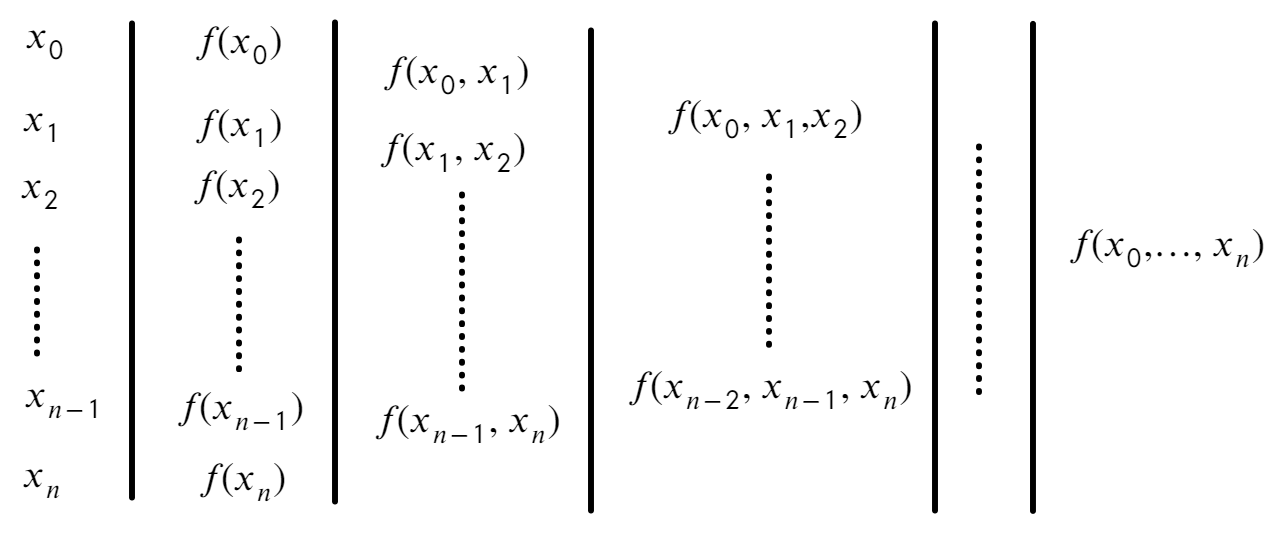
\includegraphics[scale=0.75]{img9}\]

    \begin{tcolorbox}[breakable, size=fbox, boxrule=1pt, pad at break*=1mm,colback=cellbackground, colframe=cellborder]
\prompt{In}{incolor}{36}{\boxspacing}
\begin{Verbatim}[commandchars=\\\{\}]
\PY{k}{def} \PY{n+nf}{divided\PYZus{}diff}\PY{p}{(}\PY{n}{nodes}\PY{p}{,} \PY{n}{f}\PY{p}{)}\PY{p}{:}
    \PY{n}{n} \PY{o}{=} \PY{n+nb}{len}\PY{p}{(}\PY{n}{nodes}\PY{p}{)}
    \PY{n}{divided\PYZus{}diff} \PY{o}{=} \PY{n}{np}\PY{o}{.}\PY{n}{zeros}\PY{p}{(}\PY{p}{(}\PY{n}{n}\PY{p}{,} \PY{n}{n} \PY{o}{+} \PY{l+m+mi}{1}\PY{p}{)}\PY{p}{)}

    \PY{n}{divided\PYZus{}diff}\PY{p}{[}\PY{p}{:}\PY{p}{,} \PY{l+m+mi}{0}\PY{p}{]} \PY{o}{=} \PY{p}{[}\PY{n}{f}\PY{p}{(}\PY{n}{x}\PY{p}{)} \PY{k}{for} \PY{n}{x} \PY{o+ow}{in} \PY{n}{nodes}\PY{p}{]}

    \PY{k}{for} \PY{n}{j} \PY{o+ow}{in} \PY{n+nb}{range}\PY{p}{(}\PY{l+m+mi}{1}\PY{p}{,} \PY{n}{n} \PY{o}{+} \PY{l+m+mi}{1}\PY{p}{)}\PY{p}{:}
        \PY{k}{for} \PY{n}{i} \PY{o+ow}{in} \PY{n+nb}{range}\PY{p}{(}\PY{n}{n} \PY{o}{\PYZhy{}} \PY{n}{j}\PY{p}{)}\PY{p}{:}
            \PY{n}{divided\PYZus{}diff}\PY{p}{[}\PY{n}{i}\PY{p}{,} \PY{n}{j}\PY{p}{]} \PY{o}{=} \PY{p}{(}\PY{n}{divided\PYZus{}diff}\PY{p}{[}\PY{n}{i} \PY{o}{+} \PY{l+m+mi}{1}\PY{p}{,} \PY{n}{j} \PY{o}{\PYZhy{}} \PY{l+m+mi}{1}\PY{p}{]} \PY{o}{\PYZhy{}} \PY{n}{divided\PYZus{}diff}\PY{p}{[}\PY{n}{i}\PY{p}{,} \PY{n}{j} \PY{o}{\PYZhy{}} \PY{l+m+mi}{1}\PY{p}{]}\PY{p}{)} \PY{o}{/} \PY{p}{(}\PY{n}{nodes}\PY{p}{[}\PY{n}{i} \PY{o}{+} \PY{n}{j}\PY{p}{]} \PY{o}{\PYZhy{}} \PY{n}{nodes}\PY{p}{[}\PY{n}{i}\PY{p}{]}\PY{p}{)}

    \PY{n}{divided\PYZus{}diff\PYZus{}df} \PY{o}{=} \PY{n}{pd}\PY{o}{.}\PY{n}{DataFrame}\PY{p}{(}\PY{p}{)}

    \PY{k}{for} \PY{n}{i} \PY{o+ow}{in} \PY{n+nb}{range}\PY{p}{(}\PY{n}{n}\PY{p}{)}\PY{p}{:}
        \PY{n}{divided\PYZus{}diff\PYZus{}df}\PY{o}{.}\PY{n}{loc}\PY{p}{[}\PY{p}{:}\PY{p}{,} \PY{l+s+sa}{f}\PY{l+s+s1}{\PYZsq{}}\PY{l+s+s1}{Разделенная разность порядка }\PY{l+s+si}{\PYZob{}}\PY{n}{i}\PY{+w}{ }\PY{o}{+}\PY{+w}{ }\PY{l+m+mi}{1}\PY{l+s+si}{\PYZcb{}}\PY{l+s+s1}{\PYZsq{}}\PY{p}{]} \PY{o}{=} \PY{n}{divided\PYZus{}diff}\PY{p}{[}\PY{p}{:}\PY{p}{,} \PY{n}{i}\PY{p}{]}

    \PY{n}{divided\PYZus{}diff\PYZus{}df} \PY{o}{=} \PY{n}{divided\PYZus{}diff\PYZus{}df}\PY{o}{.}\PY{n}{set\PYZus{}index}\PY{p}{(}\PY{p}{[}\PY{n}{pd}\PY{o}{.}\PY{n}{Index}\PY{p}{(}\PY{n}{nodes}\PY{p}{)}\PY{p}{]}\PY{p}{)}

    \PY{k}{return} \PY{n}{divided\PYZus{}diff\PYZus{}df}
\end{Verbatim}
\end{tcolorbox}

    Сравним значения, полученные в таблице с суммирующей функцией для,
например, 3 узлов:

    \begin{tcolorbox}[breakable, size=fbox, boxrule=1pt, pad at break*=1mm,colback=cellbackground, colframe=cellborder]
\prompt{In}{incolor}{37}{\boxspacing}
\begin{Verbatim}[commandchars=\\\{\}]
\PY{n}{nodes} \PY{o}{=} \PY{p}{[}\PY{n}{node} \PY{k}{for} \PY{n}{node} \PY{o+ow}{in} \PY{n}{interpolation\PYZus{}nodes\PYZus{}df}\PY{p}{[}\PY{l+s+s1}{\PYZsq{}}\PY{l+s+s1}{Порядок 3}\PY{l+s+s1}{\PYZsq{}}\PY{p}{]}\PY{o}{.}\PY{n}{tolist}\PY{p}{(}\PY{p}{)} \PY{k}{if} \PY{n+nb}{isinstance}\PY{p}{(}\PY{n}{node}\PY{p}{,} \PY{n+nb}{float}\PY{p}{)}\PY{p}{]}

\PY{n}{divided\PYZus{}diff}\PY{p}{(}\PY{n}{nodes}\PY{p}{,} \PY{n}{f\PYZus{}1}\PY{p}{)}
\end{Verbatim}
\end{tcolorbox}

            \begin{tcolorbox}[breakable, size=fbox, boxrule=.5pt, pad at break*=1mm, opacityfill=0]
\prompt{Out}{outcolor}{37}{\boxspacing}
\begin{Verbatim}[commandchars=\\\{\}]
            Разделенная разность порядка 1  Разделенная разность порядка 2  \textbackslash{}
-1.0000000                      -0.9893582                       0.5487816
2.0000000                        0.6569866                      -0.2219460
5.0000000                       -0.0088513                       0.0000000

            Разделенная разность порядка 3
-1.0000000                      -0.1284546
2.0000000                        0.0000000
5.0000000                        0.0000000
\end{Verbatim}
\end{tcolorbox}
        
    \begin{tcolorbox}[breakable, size=fbox, boxrule=1pt, pad at break*=1mm,colback=cellbackground, colframe=cellborder]
\prompt{In}{incolor}{38}{\boxspacing}
\begin{Verbatim}[commandchars=\\\{\}]
\PY{n}{divided\PYZus{}diff\PYZus{}sum}\PY{p}{(}\PY{n}{nodes}\PY{p}{,} \PY{n}{f\PYZus{}1}\PY{p}{)}
\end{Verbatim}
\end{tcolorbox}

            \begin{tcolorbox}[breakable, size=fbox, boxrule=.5pt, pad at break*=1mm, opacityfill=0]
\prompt{Out}{outcolor}{38}{\boxspacing}
\begin{Verbatim}[commandchars=\\\{\}]
-0.1284545974084091
\end{Verbatim}
\end{tcolorbox}
        
    Как можем видеть, разделенная разность третьего порядка, вычисленная по
формуле, совпадает с последним значением из таблицы.

Реализуем функцию для вычисления интерполяционного многочлена Ньютона.
    \[P_n(x) = f(x_0) + (x-x_0)\cdot f(x_0, x_1) + (x-x_0)(x-x_1)\cdot f(x_0,x_1,x_2) +\ldots \\ \ldots + (x-x_0)\ldots (x-x_{n-1})\cdot f(x_0,\ldots, x_n).\]

    \begin{tcolorbox}[breakable, size=fbox, boxrule=1pt, pad at break*=1mm,colback=cellbackground, colframe=cellborder]
\prompt{In}{incolor}{39}{\boxspacing}
\begin{Verbatim}[commandchars=\\\{\}]
\PY{k}{def} \PY{n+nf}{polynome\PYZus{}newton}\PY{p}{(}\PY{n}{x}\PY{p}{,} \PY{n}{nodes}\PY{p}{,} \PY{n}{div\PYZus{}diff}\PY{p}{,} \PY{n}{f}\PY{p}{)}\PY{p}{:}
    \PY{n}{p} \PY{o}{=} \PY{n}{f}\PY{p}{(}\PY{n}{nodes}\PY{p}{[}\PY{l+m+mi}{0}\PY{p}{]}\PY{p}{)}
    \PY{n}{tmp} \PY{o}{=} \PY{n}{x} \PY{o}{\PYZhy{}} \PY{n}{nodes}\PY{p}{[}\PY{l+m+mi}{0}\PY{p}{]}
    
    \PY{k}{for} \PY{n}{i} \PY{o+ow}{in} \PY{n+nb}{range}\PY{p}{(}\PY{l+m+mi}{1}\PY{p}{,} \PY{n}{n}\PY{p}{)}\PY{p}{:}
        \PY{n}{p} \PY{o}{+}\PY{o}{=} \PY{p}{(}\PY{n}{tmp} \PY{o}{*} \PY{n}{div\PYZus{}diff}\PY{p}{[}\PY{n}{i}\PY{p}{]}\PY{p}{)}
        \PY{n}{tmp} \PY{o}{*}\PY{o}{=} \PY{p}{(}\PY{n}{x} \PY{o}{\PYZhy{}} \PY{n}{nodes}\PY{p}{[}\PY{n}{i}\PY{p}{]}\PY{p}{)}
        
    \PY{k}{return} \PY{n}{p}
\end{Verbatim}
\end{tcolorbox}

    Построим графики для каждой функции \(f_1(x), f_2(x)\) для каждого из
\(n\) узлов.

    \begin{tcolorbox}[breakable, size=fbox, boxrule=1pt, pad at break*=1mm,colback=cellbackground, colframe=cellborder]
\prompt{In}{incolor}{40}{\boxspacing}
\begin{Verbatim}[commandchars=\\\{\}]
\PY{n}{x} \PY{o}{=} \PY{n}{np}\PY{o}{.}\PY{n}{linspace}\PY{p}{(}\PY{n}{a}\PY{p}{,} \PY{n}{b}\PY{p}{,} \PY{l+m+mi}{10000}\PY{p}{)}

\PY{k}{for} \PY{n}{n} \PY{o+ow}{in} \PY{p}{[}\PY{l+m+mi}{3}\PY{p}{,} \PY{l+m+mi}{5}\PY{p}{,} \PY{l+m+mi}{7}\PY{p}{,} \PY{l+m+mi}{10}\PY{p}{,} \PY{l+m+mi}{15}\PY{p}{,} \PY{l+m+mi}{20}\PY{p}{]}\PY{p}{:}
    \PY{n}{fig}\PY{p}{,} \PY{p}{(}\PY{n}{ax1}\PY{p}{,} \PY{n}{ax2}\PY{p}{)} \PY{o}{=} \PY{n}{plt}\PY{o}{.}\PY{n}{subplots}\PY{p}{(}\PY{l+m+mi}{1}\PY{p}{,} \PY{l+m+mi}{2}\PY{p}{,} \PY{n}{figsize}\PY{o}{=}\PY{p}{(}\PY{l+m+mi}{10}\PY{p}{,} \PY{l+m+mi}{4}\PY{p}{)}\PY{p}{,} \PY{n}{layout}\PY{o}{=}\PY{l+s+s1}{\PYZsq{}}\PY{l+s+s1}{constrained}\PY{l+s+s1}{\PYZsq{}}\PY{p}{,} \PY{n}{sharey}\PY{o}{=}\PY{k+kc}{False}\PY{p}{)}
    
    \PY{n}{interpolation\PYZus{}nodes} \PY{o}{=} \PY{n}{np}\PY{o}{.}\PY{n}{linspace}\PY{p}{(}\PY{n}{a}\PY{p}{,} \PY{n}{b}\PY{p}{,} \PY{n}{n}\PY{p}{)}
    \PY{n}{plot\PYZus{}dots} \PY{o}{=} \PY{n}{np}\PY{o}{.}\PY{n}{setdiff1d}\PY{p}{(}\PY{n}{x}\PY{p}{,} \PY{n}{interpolation\PYZus{}nodes}\PY{p}{)}
    
    \PY{c+c1}{\PYZsh{} построение графика функции f\PYZus{}1}
    \PY{n}{ax1}\PY{o}{.}\PY{n}{plot}\PY{p}{(}\PY{n}{x}\PY{p}{,} \PY{n}{f\PYZus{}1}\PY{p}{(}\PY{n}{x}\PY{p}{)}\PY{p}{,} \PY{n}{label}\PY{o}{=}\PY{l+s+s1}{\PYZsq{}}\PY{l+s+s1}{real function}\PY{l+s+s1}{\PYZsq{}}\PY{p}{)}
    \PY{n}{ax1}\PY{o}{.}\PY{n}{plot}\PY{p}{(}\PY{n}{plot\PYZus{}dots}\PY{p}{,} \PY{n}{polynome\PYZus{}newton}\PY{p}{(}\PY{n}{x}\PY{o}{=}\PY{n}{plot\PYZus{}dots}\PY{p}{,} \PY{n}{nodes}\PY{o}{=}\PY{n}{interpolation\PYZus{}nodes}\PY{p}{,} \PY{n}{div\PYZus{}diff}\PY{o}{=}\PY{n}{divided\PYZus{}diff}\PY{p}{(}\PY{n}{interpolation\PYZus{}nodes}\PY{p}{,} \PY{n}{f\PYZus{}1}\PY{p}{)}\PY{o}{.}\PY{n}{to\PYZus{}numpy}\PY{p}{(}\PY{p}{)}\PY{p}{[}\PY{l+m+mi}{0}\PY{p}{,} \PY{p}{:}\PY{p}{]}\PY{p}{,} \PY{n}{f}\PY{o}{=}\PY{n}{f\PYZus{}1}\PY{p}{)}\PY{p}{,} \PY{n}{label}\PY{o}{=}\PY{l+s+s1}{\PYZsq{}}\PY{l+s+s1}{interpolation}\PY{l+s+s1}{\PYZsq{}}\PY{p}{)}
    \PY{n}{ax1}\PY{o}{.}\PY{n}{set\PYZus{}xlabel}\PY{p}{(}\PY{l+s+s1}{\PYZsq{}}\PY{l+s+s1}{x}\PY{l+s+s1}{\PYZsq{}}\PY{p}{)}
    \PY{n}{ax1}\PY{o}{.}\PY{n}{set\PYZus{}ylabel}\PY{p}{(}\PY{l+s+s1}{\PYZsq{}}\PY{l+s+s1}{f(x)}\PY{l+s+s1}{\PYZsq{}}\PY{p}{)}
    \PY{n}{ax1}\PY{o}{.}\PY{n}{legend}\PY{p}{(}\PY{p}{)}
    \PY{n}{ax1}\PY{o}{.}\PY{n}{grid}\PY{p}{(}\PY{p}{)}

    \PY{c+c1}{\PYZsh{} построение графика функции f\PYZus{}2}
    \PY{n}{ax2}\PY{o}{.}\PY{n}{plot}\PY{p}{(}\PY{n}{x}\PY{p}{,} \PY{n}{f\PYZus{}2}\PY{p}{(}\PY{n}{x}\PY{p}{)}\PY{p}{,} \PY{n}{label}\PY{o}{=}\PY{l+s+s1}{\PYZsq{}}\PY{l+s+s1}{real function}\PY{l+s+s1}{\PYZsq{}}\PY{p}{)}
    \PY{n}{ax2}\PY{o}{.}\PY{n}{plot}\PY{p}{(}\PY{n}{plot\PYZus{}dots}\PY{p}{,} \PY{n}{polynome\PYZus{}newton}\PY{p}{(}\PY{n}{x}\PY{o}{=}\PY{n}{plot\PYZus{}dots}\PY{p}{,} \PY{n}{div\PYZus{}diff}\PY{o}{=}\PY{n}{divided\PYZus{}diff}\PY{p}{(}\PY{n}{interpolation\PYZus{}nodes}\PY{p}{,} \PY{n}{f\PYZus{}2}\PY{p}{)}\PY{o}{.}\PY{n}{to\PYZus{}numpy}\PY{p}{(}\PY{p}{)}\PY{p}{[}\PY{l+m+mi}{0}\PY{p}{,} \PY{p}{:}\PY{p}{]}\PY{p}{,} \PY{n}{nodes}\PY{o}{=}\PY{n}{interpolation\PYZus{}nodes}\PY{p}{,} \PY{n}{f}\PY{o}{=}\PY{n}{f\PYZus{}2}\PY{p}{)}\PY{p}{,} \PY{n}{label}\PY{o}{=}\PY{l+s+s1}{\PYZsq{}}\PY{l+s+s1}{interpolation}\PY{l+s+s1}{\PYZsq{}}\PY{p}{)}
    \PY{n}{ax2}\PY{o}{.}\PY{n}{set\PYZus{}xlabel}\PY{p}{(}\PY{l+s+s1}{\PYZsq{}}\PY{l+s+s1}{x}\PY{l+s+s1}{\PYZsq{}}\PY{p}{)}
    \PY{n}{ax2}\PY{o}{.}\PY{n}{set\PYZus{}ylabel}\PY{p}{(}\PY{l+s+s1}{\PYZsq{}}\PY{l+s+s1}{f(x)}\PY{l+s+s1}{\PYZsq{}}\PY{p}{)}
    \PY{n}{ax2}\PY{o}{.}\PY{n}{legend}\PY{p}{(}\PY{p}{)}
    \PY{n}{ax2}\PY{o}{.}\PY{n}{grid}\PY{p}{(}\PY{p}{)}

    \PY{n}{fig}\PY{o}{.}\PY{n}{suptitle}\PY{p}{(}\PY{l+s+sa}{f}\PY{l+s+s1}{\PYZsq{}}\PY{l+s+s1}{Lagrange Interpolation by }\PY{l+s+si}{\PYZob{}}\PY{n}{n}\PY{l+s+si}{\PYZcb{}}\PY{l+s+s1}{ nodes}\PY{l+s+s1}{\PYZsq{}}\PY{p}{,} \PY{n}{fontsize}\PY{o}{=}\PY{l+m+mi}{16}\PY{p}{)}
\end{Verbatim}
\end{tcolorbox}

    \begin{center}
    \adjustimage{max size={0.9\linewidth}{0.9\paperheight}}{output_73_0.png}
    \end{center}
    { \hspace*{\fill} \\}
    
    \begin{center}
    \adjustimage{max size={0.9\linewidth}{0.9\paperheight}}{output_73_1.png}
    \end{center}
    { \hspace*{\fill} \\}
    
    \begin{center}
    \adjustimage{max size={0.9\linewidth}{0.9\paperheight}}{output_73_2.png}
    \end{center}
    { \hspace*{\fill} \\}
    
    \begin{center}
    \adjustimage{max size={0.9\linewidth}{0.9\paperheight}}{output_73_3.png}
    \end{center}
    { \hspace*{\fill} \\}
    
    \begin{center}
    \adjustimage{max size={0.9\linewidth}{0.9\paperheight}}{output_73_4.png}
    \end{center}
    { \hspace*{\fill} \\}
    
    \begin{center}
    \adjustimage{max size={0.9\linewidth}{0.9\paperheight}}{output_73_5.png}
    \end{center}
    { \hspace*{\fill} \\}
    
    В соответствии с корректностью поставленной задачи, а именно
единственностью решения, мы можем увидеть, что оба интерполяционных
многочлена дали одинаковый результат, причем вне зависимости от степени
полинома. Оба они достигли наилучшего результата при \(n = 20\) узлах.
Однако в процессе построения функции всегда присутствовали отрезке
резкого отклонения.

    \subsubsection*{Интерполирование многочленами по узлам расположенным на указанном отрезке оптимальным образом}

Для минимизации остатка интерполирования выберем узлы по формуле
\[x_k = \dfrac{a+b}{2} + \dfrac{b-a}{2}\cos \dfrac{(2k+1)\pi}{2(n+1)},\ k=\overline{0,n}.\]
Если выбрать узлами интерполирования \(x_0,\ldots, x_n\) таким образом,
то величина отклонения \(\omega_{n+1}(x)\) от нуля окажется минимальной.

Для упорядочивания узлов необходима перенумерация
\(\widetilde{x}_k = x_{n-k},\ k=\overline{0,n}.\)

Составим таблицу нового разбиения на узлы.

    \begin{tcolorbox}[breakable, size=fbox, boxrule=1pt, pad at break*=1mm,colback=cellbackground, colframe=cellborder]
\prompt{In}{incolor}{41}{\boxspacing}
\begin{Verbatim}[commandchars=\\\{\}]
\PY{n}{a}\PY{p}{,} \PY{n}{b} \PY{o}{=} \PY{o}{\PYZhy{}}\PY{l+m+mi}{1}\PY{p}{,} \PY{l+m+mi}{5}

\PY{n}{interpolation\PYZus{}new\PYZus{}nodes\PYZus{}df} \PY{o}{=} \PY{n}{pd}\PY{o}{.}\PY{n}{DataFrame}\PY{p}{(}\PY{p}{)}

\PY{k}{for} \PY{n}{n} \PY{o+ow}{in} \PY{p}{[}\PY{l+m+mi}{20}\PY{p}{,} \PY{l+m+mi}{15}\PY{p}{,} \PY{l+m+mi}{10}\PY{p}{,} \PY{l+m+mi}{7}\PY{p}{,} \PY{l+m+mi}{5}\PY{p}{,} \PY{l+m+mi}{3}\PY{p}{]}\PY{p}{:}
    \PY{n}{interpolation\PYZus{}new\PYZus{}nodes\PYZus{}df}\PY{o}{.}\PY{n}{loc}\PY{p}{[}\PY{p}{:} \PY{n}{n} \PY{o}{\PYZhy{}} \PY{l+m+mi}{1}\PY{p}{,} \PY{l+s+sa}{f}\PY{l+s+s1}{\PYZsq{}}\PY{l+s+s1}{Порядок }\PY{l+s+si}{\PYZob{}}\PY{n}{n}\PY{l+s+si}{\PYZcb{}}\PY{l+s+s1}{\PYZsq{}}\PY{p}{]} \PY{o}{=} \PY{n}{np}\PY{o}{.}\PY{n}{fromiter}\PY{p}{(}\PY{p}{(}\PY{p}{(}\PY{n}{a} \PY{o}{+} \PY{n}{b}\PY{p}{)} \PY{o}{/} \PY{l+m+mi}{2} \PY{o}{+} \PY{n}{np}\PY{o}{.}\PY{n}{sum}\PY{p}{(}\PY{p}{(}\PY{n}{b} \PY{o}{\PYZhy{}} \PY{n}{a}\PY{p}{)} \PY{o}{/} \PY{l+m+mi}{2} \PY{o}{*} \PY{n}{np}\PY{o}{.}\PY{n}{cos}\PY{p}{(}\PY{p}{(}\PY{l+m+mi}{2}\PY{o}{*}\PY{n}{k} \PY{o}{+} \PY{l+m+mi}{1}\PY{p}{)} \PY{o}{*} \PY{n}{np}\PY{o}{.}\PY{n}{pi} \PY{o}{/} \PY{p}{(}\PY{l+m+mi}{2} \PY{o}{*} \PY{p}{(}\PY{n}{n} \PY{o}{+} \PY{l+m+mi}{1}\PY{p}{)}\PY{p}{)}\PY{p}{)}\PY{p}{)} \PY{k}{for} \PY{n}{k} \PY{o+ow}{in} \PY{n+nb}{range}\PY{p}{(}\PY{n}{n}\PY{p}{)}\PY{p}{)}\PY{p}{,} \PY{n}{dtype}\PY{o}{=}\PY{n+nb}{float}\PY{p}{)}\PY{p}{[}\PY{p}{:}\PY{p}{:}\PY{o}{\PYZhy{}}\PY{l+m+mi}{1}\PY{p}{]}

\PY{n}{interpolation\PYZus{}new\PYZus{}nodes\PYZus{}df} \PY{o}{=} \PY{n}{interpolation\PYZus{}new\PYZus{}nodes\PYZus{}df}\PY{o}{.}\PY{n}{fillna}\PY{p}{(}\PY{l+s+s1}{\PYZsq{}}\PY{l+s+s1}{ }\PY{l+s+s1}{\PYZsq{}}\PY{p}{)}

\PY{n}{interpolation\PYZus{}new\PYZus{}nodes\PYZus{}df}
\end{Verbatim}
\end{tcolorbox}

            \begin{tcolorbox}[breakable, size=fbox, boxrule=.5pt, pad at break*=1mm, opacityfill=0]
\prompt{Out}{outcolor}{41}{\boxspacing}
\begin{Verbatim}[commandchars=\\\{\}]
    Порядок 20 Порядок 15 Порядок 10  Порядок 7  Порядок 5 Порядок 3
0   -0.9247837 -0.8708210 -0.7288960 -0.4944088 -0.1213203 0.8519497
1   -0.7926212 -0.6457638 -0.2672487  0.3332893  1.2235429 3.1480503
2   -0.5980762 -0.3190314  0.3780775  1.4147290  2.7764571 4.7716386
3   -0.3454944  0.0968201  1.1548023  2.5852710  4.1213203
4   -0.0405182  0.5858098  2.0000000  3.6667107  4.8977775
5    0.3100398  1.1291460  2.8451977  4.4944088
6    0.6983488  1.7059486  3.6219225  4.9423558
7    1.1157345  2.2940514  4.2672487
8    1.5528732  2.8708540  4.7288960
9    2.0000000  3.4141902  4.9694643
10   2.4471268  3.9031799
11   2.8842655  4.3190314
12   3.3016512  4.6457638
13   3.6899602  4.8708210
14   4.0405182  4.9855542
15   4.3454944
16   4.5980762
17   4.7926212
18   4.9247837
19   4.9916114
\end{Verbatim}
\end{tcolorbox}
        
    Будем действовать в том же порядке, сначала рассмотрим интерполирование
многочленом Лагранжа.

    \begin{tcolorbox}[breakable, size=fbox, boxrule=1pt, pad at break*=1mm,colback=cellbackground, colframe=cellborder]
\prompt{In}{incolor}{42}{\boxspacing}
\begin{Verbatim}[commandchars=\\\{\}]
\PY{n}{x} \PY{o}{=} \PY{n}{np}\PY{o}{.}\PY{n}{linspace}\PY{p}{(}\PY{n}{a}\PY{p}{,} \PY{n}{b}\PY{p}{,} \PY{l+m+mi}{10000}\PY{p}{)}

\PY{k}{for} \PY{n}{n} \PY{o+ow}{in} \PY{p}{[}\PY{l+m+mi}{3}\PY{p}{,} \PY{l+m+mi}{5}\PY{p}{,} \PY{l+m+mi}{7}\PY{p}{,} \PY{l+m+mi}{10}\PY{p}{,} \PY{l+m+mi}{15}\PY{p}{,} \PY{l+m+mi}{20}\PY{p}{]}\PY{p}{:}
    \PY{n}{fig}\PY{p}{,} \PY{p}{(}\PY{n}{ax1}\PY{p}{,} \PY{n}{ax2}\PY{p}{)} \PY{o}{=} \PY{n}{plt}\PY{o}{.}\PY{n}{subplots}\PY{p}{(}\PY{l+m+mi}{1}\PY{p}{,} \PY{l+m+mi}{2}\PY{p}{,} \PY{n}{figsize}\PY{o}{=}\PY{p}{(}\PY{l+m+mi}{10}\PY{p}{,} \PY{l+m+mi}{4}\PY{p}{)}\PY{p}{,} \PY{n}{layout}\PY{o}{=}\PY{l+s+s1}{\PYZsq{}}\PY{l+s+s1}{constrained}\PY{l+s+s1}{\PYZsq{}}\PY{p}{,} \PY{n}{sharey}\PY{o}{=}\PY{k+kc}{False}\PY{p}{)}
    
    \PY{n}{interpolation\PYZus{}nodes} \PY{o}{=} \PY{p}{[}\PY{n}{node} \PY{k}{for} \PY{n}{node} \PY{o+ow}{in} \PY{n}{interpolation\PYZus{}new\PYZus{}nodes\PYZus{}df}\PY{p}{[}\PY{l+s+sa}{f}\PY{l+s+s1}{\PYZsq{}}\PY{l+s+s1}{Порядок }\PY{l+s+si}{\PYZob{}}\PY{n}{n}\PY{l+s+si}{\PYZcb{}}\PY{l+s+s1}{\PYZsq{}}\PY{p}{]}\PY{o}{.}\PY{n}{tolist}\PY{p}{(}\PY{p}{)} \PY{k}{if} \PY{n+nb}{isinstance}\PY{p}{(}\PY{n}{node}\PY{p}{,} \PY{n+nb}{float}\PY{p}{)}\PY{p}{]}
    \PY{n}{plot\PYZus{}dots} \PY{o}{=} \PY{n}{np}\PY{o}{.}\PY{n}{setdiff1d}\PY{p}{(}\PY{n}{x}\PY{p}{,} \PY{n}{interpolation\PYZus{}nodes}\PY{p}{)}
    
    \PY{c+c1}{\PYZsh{} построение графика функции f\PYZus{}1}
    \PY{n}{ax1}\PY{o}{.}\PY{n}{plot}\PY{p}{(}\PY{n}{x}\PY{p}{,} \PY{n}{f\PYZus{}1}\PY{p}{(}\PY{n}{x}\PY{p}{)}\PY{p}{,} \PY{n}{label}\PY{o}{=}\PY{l+s+s1}{\PYZsq{}}\PY{l+s+s1}{real function}\PY{l+s+s1}{\PYZsq{}}\PY{p}{)}
    \PY{n}{ax1}\PY{o}{.}\PY{n}{plot}\PY{p}{(}\PY{n}{plot\PYZus{}dots}\PY{p}{,} \PY{n}{polynome\PYZus{}lagrange}\PY{p}{(}\PY{n}{x}\PY{o}{=}\PY{n}{plot\PYZus{}dots}\PY{p}{,} \PY{n}{nodes}\PY{o}{=}\PY{n}{interpolation\PYZus{}nodes}\PY{p}{,} \PY{n}{f}\PY{o}{=}\PY{n}{f\PYZus{}1}\PY{p}{)}\PY{p}{,} \PY{n}{label}\PY{o}{=}\PY{l+s+s1}{\PYZsq{}}\PY{l+s+s1}{interpolation}\PY{l+s+s1}{\PYZsq{}}\PY{p}{)}
    \PY{n}{ax1}\PY{o}{.}\PY{n}{set\PYZus{}xlabel}\PY{p}{(}\PY{l+s+s1}{\PYZsq{}}\PY{l+s+s1}{x}\PY{l+s+s1}{\PYZsq{}}\PY{p}{)}
    \PY{n}{ax1}\PY{o}{.}\PY{n}{set\PYZus{}ylabel}\PY{p}{(}\PY{l+s+s1}{\PYZsq{}}\PY{l+s+s1}{f(x)}\PY{l+s+s1}{\PYZsq{}}\PY{p}{)}
    \PY{n}{ax1}\PY{o}{.}\PY{n}{legend}\PY{p}{(}\PY{p}{)}
    \PY{n}{ax1}\PY{o}{.}\PY{n}{grid}\PY{p}{(}\PY{p}{)}

    \PY{c+c1}{\PYZsh{} построение графика функции f\PYZus{}2}
    \PY{n}{ax2}\PY{o}{.}\PY{n}{plot}\PY{p}{(}\PY{n}{x}\PY{p}{,} \PY{n}{f\PYZus{}2}\PY{p}{(}\PY{n}{x}\PY{p}{)}\PY{p}{,} \PY{n}{label}\PY{o}{=}\PY{l+s+s1}{\PYZsq{}}\PY{l+s+s1}{real function}\PY{l+s+s1}{\PYZsq{}}\PY{p}{)}
    \PY{n}{ax2}\PY{o}{.}\PY{n}{plot}\PY{p}{(}\PY{n}{plot\PYZus{}dots}\PY{p}{,} \PY{n}{polynome\PYZus{}lagrange}\PY{p}{(}\PY{n}{x}\PY{o}{=}\PY{n}{plot\PYZus{}dots}\PY{p}{,} \PY{n}{nodes}\PY{o}{=}\PY{n}{interpolation\PYZus{}nodes}\PY{p}{,} \PY{n}{f}\PY{o}{=}\PY{n}{f\PYZus{}2}\PY{p}{)}\PY{p}{,} \PY{n}{label}\PY{o}{=}\PY{l+s+s1}{\PYZsq{}}\PY{l+s+s1}{interpolation}\PY{l+s+s1}{\PYZsq{}}\PY{p}{)}
    \PY{n}{ax2}\PY{o}{.}\PY{n}{set\PYZus{}xlabel}\PY{p}{(}\PY{l+s+s1}{\PYZsq{}}\PY{l+s+s1}{x}\PY{l+s+s1}{\PYZsq{}}\PY{p}{)}
    \PY{n}{ax2}\PY{o}{.}\PY{n}{set\PYZus{}ylabel}\PY{p}{(}\PY{l+s+s1}{\PYZsq{}}\PY{l+s+s1}{f(x)}\PY{l+s+s1}{\PYZsq{}}\PY{p}{)}
    \PY{n}{ax2}\PY{o}{.}\PY{n}{legend}\PY{p}{(}\PY{p}{)}
    \PY{n}{ax2}\PY{o}{.}\PY{n}{grid}\PY{p}{(}\PY{p}{)}

    \PY{n}{fig}\PY{o}{.}\PY{n}{suptitle}\PY{p}{(}\PY{l+s+sa}{f}\PY{l+s+s1}{\PYZsq{}}\PY{l+s+s1}{Lagrange Interpolation by }\PY{l+s+si}{\PYZob{}}\PY{n}{n}\PY{l+s+si}{\PYZcb{}}\PY{l+s+s1}{ nodes}\PY{l+s+s1}{\PYZsq{}}\PY{p}{,} \PY{n}{fontsize}\PY{o}{=}\PY{l+m+mi}{16}\PY{p}{)}
\end{Verbatim}
\end{tcolorbox}


    \begin{center}
    \adjustimage{max size={0.9\linewidth}{0.9\paperheight}}{output_78_1.png}
    \end{center}
    { \hspace*{\fill} \\}
    
    \begin{center}
    \adjustimage{max size={0.9\linewidth}{0.9\paperheight}}{output_78_2.png}
    \end{center}
    { \hspace*{\fill} \\}
    
    \begin{center}
    \adjustimage{max size={0.9\linewidth}{0.9\paperheight}}{output_78_3.png}
    \end{center}
    { \hspace*{\fill} \\}
    
    \begin{center}
    \adjustimage{max size={0.9\linewidth}{0.9\paperheight}}{output_78_4.png}
    \end{center}
    { \hspace*{\fill} \\}
    
    \begin{center}
    \adjustimage{max size={0.9\linewidth}{0.9\paperheight}}{output_78_5.png}
    \end{center}
    { \hspace*{\fill} \\}
    
    \begin{center}
    \adjustimage{max size={0.9\linewidth}{0.9\paperheight}}{output_78_6.png}
    \end{center}
    { \hspace*{\fill} \\}
    
    Теперь рассмотрим интерполирование многочленом Ньютона.

    \begin{tcolorbox}[breakable, size=fbox, boxrule=1pt, pad at break*=1mm,colback=cellbackground, colframe=cellborder]
\prompt{In}{incolor}{43}{\boxspacing}
\begin{Verbatim}[commandchars=\\\{\}]
\PY{n}{x} \PY{o}{=} \PY{n}{np}\PY{o}{.}\PY{n}{linspace}\PY{p}{(}\PY{n}{a}\PY{p}{,} \PY{n}{b}\PY{p}{,} \PY{l+m+mi}{10000}\PY{p}{)}

\PY{k}{for} \PY{n}{n} \PY{o+ow}{in} \PY{p}{[}\PY{l+m+mi}{3}\PY{p}{,} \PY{l+m+mi}{5}\PY{p}{,} \PY{l+m+mi}{7}\PY{p}{,} \PY{l+m+mi}{10}\PY{p}{,} \PY{l+m+mi}{15}\PY{p}{,} \PY{l+m+mi}{20}\PY{p}{]}\PY{p}{:}
    \PY{n}{fig}\PY{p}{,} \PY{p}{(}\PY{n}{ax1}\PY{p}{,} \PY{n}{ax2}\PY{p}{)} \PY{o}{=} \PY{n}{plt}\PY{o}{.}\PY{n}{subplots}\PY{p}{(}\PY{l+m+mi}{1}\PY{p}{,} \PY{l+m+mi}{2}\PY{p}{,} \PY{n}{figsize}\PY{o}{=}\PY{p}{(}\PY{l+m+mi}{10}\PY{p}{,} \PY{l+m+mi}{4}\PY{p}{)}\PY{p}{,} \PY{n}{layout}\PY{o}{=}\PY{l+s+s1}{\PYZsq{}}\PY{l+s+s1}{constrained}\PY{l+s+s1}{\PYZsq{}}\PY{p}{,} \PY{n}{sharey}\PY{o}{=}\PY{k+kc}{False}\PY{p}{)}
    
    \PY{n}{interpolation\PYZus{}nodes} \PY{o}{=} \PY{p}{[}\PY{n}{node} \PY{k}{for} \PY{n}{node} \PY{o+ow}{in} \PY{n}{interpolation\PYZus{}new\PYZus{}nodes\PYZus{}df}\PY{p}{[}\PY{l+s+sa}{f}\PY{l+s+s1}{\PYZsq{}}\PY{l+s+s1}{Порядок }\PY{l+s+si}{\PYZob{}}\PY{n}{n}\PY{l+s+si}{\PYZcb{}}\PY{l+s+s1}{\PYZsq{}}\PY{p}{]}\PY{o}{.}\PY{n}{tolist}\PY{p}{(}\PY{p}{)} \PY{k}{if} \PY{n+nb}{isinstance}\PY{p}{(}\PY{n}{node}\PY{p}{,} \PY{n+nb}{float}\PY{p}{)}\PY{p}{]}
    \PY{n}{plot\PYZus{}dots} \PY{o}{=} \PY{n}{np}\PY{o}{.}\PY{n}{setdiff1d}\PY{p}{(}\PY{n}{x}\PY{p}{,} \PY{n}{interpolation\PYZus{}nodes}\PY{p}{)}
    
    \PY{c+c1}{\PYZsh{} построение графика функции f\PYZus{}1}
    \PY{n}{ax1}\PY{o}{.}\PY{n}{plot}\PY{p}{(}\PY{n}{x}\PY{p}{,} \PY{n}{f\PYZus{}1}\PY{p}{(}\PY{n}{x}\PY{p}{)}\PY{p}{,} \PY{n}{label}\PY{o}{=}\PY{l+s+s1}{\PYZsq{}}\PY{l+s+s1}{real function}\PY{l+s+s1}{\PYZsq{}}\PY{p}{)}
    \PY{n}{ax1}\PY{o}{.}\PY{n}{plot}\PY{p}{(}\PY{n}{plot\PYZus{}dots}\PY{p}{,} \PY{n}{polynome\PYZus{}newton}\PY{p}{(}\PY{n}{x}\PY{o}{=}\PY{n}{plot\PYZus{}dots}\PY{p}{,} \PY{n}{nodes}\PY{o}{=}\PY{n}{interpolation\PYZus{}nodes}\PY{p}{,} \PY{n}{div\PYZus{}diff}\PY{o}{=}\PY{n}{divided\PYZus{}diff}\PY{p}{(}\PY{n}{interpolation\PYZus{}nodes}\PY{p}{,} \PY{n}{f\PYZus{}1}\PY{p}{)}\PY{o}{.}\PY{n}{to\PYZus{}numpy}\PY{p}{(}\PY{p}{)}\PY{p}{[}\PY{l+m+mi}{0}\PY{p}{,} \PY{p}{:}\PY{p}{]}\PY{p}{,} \PY{n}{f}\PY{o}{=}\PY{n}{f\PYZus{}1}\PY{p}{)}\PY{p}{,} \PY{n}{label}\PY{o}{=}\PY{l+s+s1}{\PYZsq{}}\PY{l+s+s1}{interpolation}\PY{l+s+s1}{\PYZsq{}}\PY{p}{)}
    \PY{n}{ax1}\PY{o}{.}\PY{n}{set\PYZus{}xlabel}\PY{p}{(}\PY{l+s+s1}{\PYZsq{}}\PY{l+s+s1}{x}\PY{l+s+s1}{\PYZsq{}}\PY{p}{)}
    \PY{n}{ax1}\PY{o}{.}\PY{n}{set\PYZus{}ylabel}\PY{p}{(}\PY{l+s+s1}{\PYZsq{}}\PY{l+s+s1}{f(x)}\PY{l+s+s1}{\PYZsq{}}\PY{p}{)}
    \PY{n}{ax1}\PY{o}{.}\PY{n}{legend}\PY{p}{(}\PY{p}{)}
    \PY{n}{ax1}\PY{o}{.}\PY{n}{grid}\PY{p}{(}\PY{p}{)}

    \PY{c+c1}{\PYZsh{} построение графика функции f\PYZus{}2}
    \PY{n}{ax2}\PY{o}{.}\PY{n}{plot}\PY{p}{(}\PY{n}{x}\PY{p}{,} \PY{n}{f\PYZus{}2}\PY{p}{(}\PY{n}{x}\PY{p}{)}\PY{p}{,} \PY{n}{label}\PY{o}{=}\PY{l+s+s1}{\PYZsq{}}\PY{l+s+s1}{real function}\PY{l+s+s1}{\PYZsq{}}\PY{p}{)}
    \PY{n}{ax2}\PY{o}{.}\PY{n}{plot}\PY{p}{(}\PY{n}{plot\PYZus{}dots}\PY{p}{,} \PY{n}{polynome\PYZus{}newton}\PY{p}{(}\PY{n}{x}\PY{o}{=}\PY{n}{plot\PYZus{}dots}\PY{p}{,} \PY{n}{div\PYZus{}diff}\PY{o}{=}\PY{n}{divided\PYZus{}diff}\PY{p}{(}\PY{n}{interpolation\PYZus{}nodes}\PY{p}{,} \PY{n}{f\PYZus{}2}\PY{p}{)}\PY{o}{.}\PY{n}{to\PYZus{}numpy}\PY{p}{(}\PY{p}{)}\PY{p}{[}\PY{l+m+mi}{0}\PY{p}{,} \PY{p}{:}\PY{p}{]}\PY{p}{,} \PY{n}{nodes}\PY{o}{=}\PY{n}{interpolation\PYZus{}nodes}\PY{p}{,} \PY{n}{f}\PY{o}{=}\PY{n}{f\PYZus{}2}\PY{p}{)}\PY{p}{,} \PY{n}{label}\PY{o}{=}\PY{l+s+s1}{\PYZsq{}}\PY{l+s+s1}{interpolation}\PY{l+s+s1}{\PYZsq{}}\PY{p}{)}
    \PY{n}{ax2}\PY{o}{.}\PY{n}{set\PYZus{}xlabel}\PY{p}{(}\PY{l+s+s1}{\PYZsq{}}\PY{l+s+s1}{x}\PY{l+s+s1}{\PYZsq{}}\PY{p}{)}
    \PY{n}{ax2}\PY{o}{.}\PY{n}{set\PYZus{}ylabel}\PY{p}{(}\PY{l+s+s1}{\PYZsq{}}\PY{l+s+s1}{f(x)}\PY{l+s+s1}{\PYZsq{}}\PY{p}{)}
    \PY{n}{ax2}\PY{o}{.}\PY{n}{legend}\PY{p}{(}\PY{p}{)}
    \PY{n}{ax2}\PY{o}{.}\PY{n}{grid}\PY{p}{(}\PY{p}{)}

    \PY{n}{fig}\PY{o}{.}\PY{n}{suptitle}\PY{p}{(}\PY{l+s+sa}{f}\PY{l+s+s1}{\PYZsq{}}\PY{l+s+s1}{Lagrange Interpolation by }\PY{l+s+si}{\PYZob{}}\PY{n}{n}\PY{l+s+si}{\PYZcb{}}\PY{l+s+s1}{ nodes}\PY{l+s+s1}{\PYZsq{}}\PY{p}{,} \PY{n}{fontsize}\PY{o}{=}\PY{l+m+mi}{16}\PY{p}{)}
\end{Verbatim}
\end{tcolorbox}

    \begin{center}
    \adjustimage{max size={0.9\linewidth}{0.9\paperheight}}{output_80_0.png}
    \end{center}
    { \hspace*{\fill} \\}
    
    \begin{center}
    \adjustimage{max size={0.9\linewidth}{0.9\paperheight}}{output_80_1.png}
    \end{center}
    { \hspace*{\fill} \\}
    
    \begin{center}
    \adjustimage{max size={0.9\linewidth}{0.9\paperheight}}{output_80_2.png}
    \end{center}
    { \hspace*{\fill} \\}
    
    \begin{center}
    \adjustimage{max size={0.9\linewidth}{0.9\paperheight}}{output_80_3.png}
    \end{center}
    { \hspace*{\fill} \\}
    
    \begin{center}
    \adjustimage{max size={0.9\linewidth}{0.9\paperheight}}{output_80_4.png}
    \end{center}
    { \hspace*{\fill} \\}
    
    \begin{center}
    \adjustimage{max size={0.9\linewidth}{0.9\paperheight}}{output_80_5.png}
    \end{center}
    { \hspace*{\fill} \\}
    
    В целом, аналогично раномерному распределению узлов по отрезку, получаем
то, что результат интерполирования не отличается от выбора вида
полинома. Однако в этом случае результат стал немного лучше как для
функции \(f_1(x)\) так и для \(f_2(x)\). Стоит обратить внимание на то,
что для обеих функций пристуствуют отрезке резкого отклонения как для
полинома Лагранжа, так и для полинома Ньютона.

    \subsubsection*{Вывод}

По итогам выполнения задания 2 можно сделать вывод, что для заданных
функций \(f_1(x) = \sin{(5x-3)} \ \text{и} \ f_2(x) = |2x-3|\) лучшим
образом работает интерполирования по узлам, расположенным оптимальным
образом, причем для \(f_1(x)\) результат точнее. Наличие отрезков, где
наблюдаются сильные различия можно обусловить простым недостатком узлов,
возможно, при использовании \(30\) узлов, результат будет лучше.
Проверим это

    \begin{tcolorbox}[breakable, size=fbox, boxrule=1pt, pad at break*=1mm,colback=cellbackground, colframe=cellborder]
\prompt{In}{incolor}{44}{\boxspacing}
\begin{Verbatim}[commandchars=\\\{\}]
\PY{n}{a}\PY{p}{,} \PY{n}{b} \PY{o}{=} \PY{o}{\PYZhy{}}\PY{l+m+mi}{1}\PY{p}{,} \PY{l+m+mi}{5}

\PY{n}{interpolation\PYZus{}node} \PY{o}{=} \PY{p}{[}\PY{p}{]}

\PY{n}{n} \PY{o}{=} \PY{l+m+mi}{30}

\PY{n}{interpolation\PYZus{}node} \PY{o}{=}  \PY{n}{np}\PY{o}{.}\PY{n}{fromiter}\PY{p}{(}\PY{p}{(}\PY{p}{(}\PY{n}{a} \PY{o}{+} \PY{n}{b}\PY{p}{)} \PY{o}{/} \PY{l+m+mi}{2} \PY{o}{+} \PY{n}{np}\PY{o}{.}\PY{n}{sum}\PY{p}{(}\PY{p}{(}\PY{n}{b} \PY{o}{\PYZhy{}} \PY{n}{a}\PY{p}{)} \PY{o}{/} \PY{l+m+mi}{2} \PY{o}{*} \PY{n}{np}\PY{o}{.}\PY{n}{cos}\PY{p}{(}\PY{p}{(}\PY{l+m+mi}{2}\PY{o}{*}\PY{n}{k} \PY{o}{+} \PY{l+m+mi}{1}\PY{p}{)} \PY{o}{*} \PY{n}{np}\PY{o}{.}\PY{n}{pi} \PY{o}{/} \PY{p}{(}\PY{l+m+mi}{2} \PY{o}{*} \PY{p}{(}\PY{n}{n} \PY{o}{+} \PY{l+m+mi}{1}\PY{p}{)}\PY{p}{)}\PY{p}{)}\PY{p}{)} \PY{k}{for} \PY{n}{k} \PY{o+ow}{in} \PY{n+nb}{range}\PY{p}{(}\PY{n}{n}\PY{p}{)}\PY{p}{)}\PY{p}{,} \PY{n}{dtype}\PY{o}{=}\PY{n+nb}{float}\PY{p}{)}\PY{p}{[}\PY{p}{:}\PY{p}{:}\PY{o}{\PYZhy{}}\PY{l+m+mi}{1}\PY{p}{]}

\PY{n}{interpolation\PYZus{}node}
\end{Verbatim}
\end{tcolorbox}

            \begin{tcolorbox}[breakable, size=fbox, boxrule=.5pt, pad at break*=1mm, opacityfill=0]
\prompt{Out}{outcolor}{44}{\boxspacing}
\begin{Verbatim}[commandchars=\\\{\}]
array([-0.96540497, -0.90423136, -0.8132564 , -0.69341362, -0.54593277,
       -0.37232721, -0.17437836,  0.04588255,  0.28619535,  0.54409411,
        0.81693243,  1.10191063,  1.39610444,  1.69649503,  2.        ,
        2.30350497,  2.60389556,  2.89808937,  3.18306757,  3.45590589,
        3.71380465,  3.95411745,  4.17437836,  4.37232721,  4.54593277,
        4.69341362,  4.8132564 ,  4.90423136,  4.96540497,  4.99614952])
\end{Verbatim}
\end{tcolorbox}
        
    \begin{tcolorbox}[breakable, size=fbox, boxrule=1pt, pad at break*=1mm,colback=cellbackground, colframe=cellborder]
\prompt{In}{incolor}{45}{\boxspacing}
\begin{Verbatim}[commandchars=\\\{\}]
\PY{n}{x} \PY{o}{=} \PY{n}{np}\PY{o}{.}\PY{n}{linspace}\PY{p}{(}\PY{n}{a}\PY{p}{,} \PY{n}{b}\PY{p}{,} \PY{l+m+mi}{10000}\PY{p}{)}

\PY{n}{fig}\PY{p}{,} \PY{p}{(}\PY{n}{ax1}\PY{p}{,} \PY{n}{ax2}\PY{p}{)} \PY{o}{=} \PY{n}{plt}\PY{o}{.}\PY{n}{subplots}\PY{p}{(}\PY{l+m+mi}{1}\PY{p}{,} \PY{l+m+mi}{2}\PY{p}{,} \PY{n}{figsize}\PY{o}{=}\PY{p}{(}\PY{l+m+mi}{10}\PY{p}{,} \PY{l+m+mi}{4}\PY{p}{)}\PY{p}{,} \PY{n}{layout}\PY{o}{=}\PY{l+s+s1}{\PYZsq{}}\PY{l+s+s1}{constrained}\PY{l+s+s1}{\PYZsq{}}\PY{p}{,} \PY{n}{sharey}\PY{o}{=}\PY{k+kc}{False}\PY{p}{)}
    
\PY{n}{plot\PYZus{}dots} \PY{o}{=} \PY{n}{np}\PY{o}{.}\PY{n}{setdiff1d}\PY{p}{(}\PY{n}{x}\PY{p}{,} \PY{n}{interpolation\PYZus{}node}\PY{p}{)}
    
\PY{c+c1}{\PYZsh{} построение графика функции f\PYZus{}1}
\PY{n}{ax1}\PY{o}{.}\PY{n}{plot}\PY{p}{(}\PY{n}{x}\PY{p}{,} \PY{n}{f\PYZus{}1}\PY{p}{(}\PY{n}{x}\PY{p}{)}\PY{p}{,} \PY{n}{label}\PY{o}{=}\PY{l+s+s1}{\PYZsq{}}\PY{l+s+s1}{real function}\PY{l+s+s1}{\PYZsq{}}\PY{p}{)}
\PY{n}{ax1}\PY{o}{.}\PY{n}{plot}\PY{p}{(}\PY{n}{plot\PYZus{}dots}\PY{p}{,} \PY{n}{polynome\PYZus{}lagrange}\PY{p}{(}\PY{n}{x}\PY{o}{=}\PY{n}{plot\PYZus{}dots}\PY{p}{,} \PY{n}{nodes}\PY{o}{=}\PY{n}{interpolation\PYZus{}node}\PY{p}{,} \PY{n}{f}\PY{o}{=}\PY{n}{f\PYZus{}1}\PY{p}{)}\PY{p}{,} \PY{n}{label}\PY{o}{=}\PY{l+s+s1}{\PYZsq{}}\PY{l+s+s1}{interpolation}\PY{l+s+s1}{\PYZsq{}}\PY{p}{)}
\PY{n}{ax1}\PY{o}{.}\PY{n}{set\PYZus{}xlabel}\PY{p}{(}\PY{l+s+s1}{\PYZsq{}}\PY{l+s+s1}{x}\PY{l+s+s1}{\PYZsq{}}\PY{p}{)}
\PY{n}{ax1}\PY{o}{.}\PY{n}{set\PYZus{}ylabel}\PY{p}{(}\PY{l+s+s1}{\PYZsq{}}\PY{l+s+s1}{f(x)}\PY{l+s+s1}{\PYZsq{}}\PY{p}{)}
\PY{n}{ax1}\PY{o}{.}\PY{n}{legend}\PY{p}{(}\PY{p}{)}
\PY{n}{ax1}\PY{o}{.}\PY{n}{grid}\PY{p}{(}\PY{p}{)}

\PY{c+c1}{\PYZsh{} построение графика функции f\PYZus{}2}
\PY{n}{ax2}\PY{o}{.}\PY{n}{plot}\PY{p}{(}\PY{n}{x}\PY{p}{,} \PY{n}{f\PYZus{}2}\PY{p}{(}\PY{n}{x}\PY{p}{)}\PY{p}{,} \PY{n}{label}\PY{o}{=}\PY{l+s+s1}{\PYZsq{}}\PY{l+s+s1}{real function}\PY{l+s+s1}{\PYZsq{}}\PY{p}{)}
\PY{n}{ax2}\PY{o}{.}\PY{n}{plot}\PY{p}{(}\PY{n}{plot\PYZus{}dots}\PY{p}{,} \PY{n}{polynome\PYZus{}lagrange}\PY{p}{(}\PY{n}{x}\PY{o}{=}\PY{n}{plot\PYZus{}dots}\PY{p}{,} \PY{n}{nodes}\PY{o}{=}\PY{n}{interpolation\PYZus{}node}\PY{p}{,} \PY{n}{f}\PY{o}{=}\PY{n}{f\PYZus{}2}\PY{p}{)}\PY{p}{,} \PY{n}{label}\PY{o}{=}\PY{l+s+s1}{\PYZsq{}}\PY{l+s+s1}{interpolation}\PY{l+s+s1}{\PYZsq{}}\PY{p}{)}
\PY{n}{ax2}\PY{o}{.}\PY{n}{set\PYZus{}xlabel}\PY{p}{(}\PY{l+s+s1}{\PYZsq{}}\PY{l+s+s1}{x}\PY{l+s+s1}{\PYZsq{}}\PY{p}{)}
\PY{n}{ax2}\PY{o}{.}\PY{n}{set\PYZus{}ylabel}\PY{p}{(}\PY{l+s+s1}{\PYZsq{}}\PY{l+s+s1}{f(x)}\PY{l+s+s1}{\PYZsq{}}\PY{p}{)}
\PY{n}{ax2}\PY{o}{.}\PY{n}{legend}\PY{p}{(}\PY{p}{)}
\PY{n}{ax2}\PY{o}{.}\PY{n}{grid}\PY{p}{(}\PY{p}{)}

\PY{n}{fig}\PY{o}{.}\PY{n}{suptitle}\PY{p}{(}\PY{l+s+sa}{f}\PY{l+s+s1}{\PYZsq{}}\PY{l+s+s1}{Lagrange Interpolation by }\PY{l+s+si}{\PYZob{}}\PY{n}{n}\PY{l+s+si}{\PYZcb{}}\PY{l+s+s1}{ nodes}\PY{l+s+s1}{\PYZsq{}}\PY{p}{,} \PY{n}{fontsize}\PY{o}{=}\PY{l+m+mi}{16}\PY{p}{)}
\end{Verbatim}
\end{tcolorbox}

        
    \begin{center}
    \adjustimage{max size={0.9\linewidth}{0.9\paperheight}}{output_84_2.png}
    \end{center}
    { \hspace*{\fill} \\}
    
    При использовании \(30\) узлов, интерполирование Лагранжа работает
идеально для функции \(f_1(x) =\sin(5x - 3)\), а для функции
\(f_2(x) = |2x - 3|\) всё еще есть недочеты.
    
\end{document}
